\documentclass{beamer}
\usepackage[export]{adjustbox}
\usepackage{booktabs}
\usepackage{caption}
\usepackage{fancyvrb}
\usepackage{graphicx}
\usepackage{mathtools}
\usepackage{pdfpages}
\usepackage{siunitx}
\usepackage{tikz}
\usetikzlibrary{positioning}
\usepackage{xcolor}
\usepackage{xspace}

\setbeamertemplate{navigation symbols}{} %turn off navigation symbols

\makeatother
\setbeamertemplate{footline}
{
	\leavevmode%
	\hbox{%
		\begin{beamercolorbox}[wd=0.3\paperwidth,left]{white}
			\usebeamerfont{author in head/foot}\insertshortauthor
		\end{beamercolorbox}
    	\begin{beamercolorbox}[wd=0.4\paperwidth,center]{white}
    		\usebeamerfont{title in head/foot}\textbf{\insertshorttitle: \insertshortsubtitle}
    	\end{beamercolorbox}
    	\begin{beamercolorbox}[wd=0.3\paperwidth,right]{white}
    		\insertframenumber{} / \inserttotalframenumber
    	\end{beamercolorbox}
    }%
  	\vskip0pt%
}
\makeatletter
%\setbeamertemplate{footline}[frame number]


\title{Summer oscillation analysis}
\subtitle{VALOR update}

\author{\textbf{Chris Barry}, Andy Chappell}
\institute{     
\includegraphics[height=1.2cm]{images/t2k_logo_medium}\\
\includegraphics[width=0.3\textwidth,keepaspectratio]{images/University_of_Liverpool_logo}
\hspace*{1cm}

\includegraphics[width=0.23\textwidth,keepaspectratio]{images/warwick_logo}
}
\date{23 May 2017}

\newcommand{\deltacp}{$\delta_{CP}$\xspace}
\newcommand{\sinsqthetaonethree}{$\sin^2\theta_{13}$\xspace}
\newcommand{\sinsqthetatwothree}{$\sin^2\theta_{23}$\xspace}
\newcommand{\dmsqtwothree}{$\Delta m^2_{23}$\xspace}

\begin{document}

\begin{frame}
	\titlepage
\end{frame}

%===============================================================================
\section*{VALOR Status}
\begin{frame}{VALOR status}
	\begin{itemize}
		\item Event rates show good agreement with p-theta and MaCh3
		\item Systematic variations show good agreement with p-theta and MaCh3
		\item Statistics only Asimov fits between VALOR and p-theta agree
		\item Asimov fits shown today use May 04 BANFF matrix
		\begin{itemize}
			\item Does not include bug fixes referred to in Clarence's talk
			\item All plots should be considered preliminary
		\end{itemize}
		\item Tech note near complete pending final results
	\end{itemize}
\end{frame}

%===============================================================================
\section*{Asimov definitions}
\begin{frame}{Asimov definitions}
	\centering
	\begin{tabular}{| c | c | c |}
	\hline
	Parameter(s) &	Asimov A & Asimov B	\\
	\hline
	$\sin^{2} \theta_{12}$	&	0.304	&	0.304	\\
	$\sin^{2}\theta_{23}$	&	0.528	&  0.624	\\
	$\sin^{2} \theta_{13}$	&	0.0217	&	0.0217	\\
	$\Delta m^{2}_{21}$	&	$7.53 \times 10^{-5}~\mbox{eV}^2/\mbox{c}^4$	&	$7.53 \times 10^{-5}~\mbox{eV}^2/\mbox{c}^4$	\\
	$\Delta m^{2}_{32}$ 	&	$2.509 \times 10^{-3}~\mbox{eV}^2/\mbox{c}^4$	&	$2.509 \times 10^{-3}~\mbox{eV}^2/\mbox{c}^4$	\\
	$\delta_{CP}$	&	-1.601	&	0	\\
	Mass Hierarchy	&	Normal	&	Normal	\\  
	\hline
	\end{tabular} %
	\begin{itemize}
		\item Asimov A based on T2K Run 1-7 best fit
		\item Asimov B uses NOvA non-maximal $\theta_{23}$ and CP conservation
	\end{itemize}
\end{frame}

%===============================================================================
\section{Event rates}
\begin{frame}
	\centering
	\Large Run 1-8 event rates
\end{frame}

\begin{frame}{Total event rates by mode}
	\centering
	\begin{tabular}{ | l || r | r | }
		\hline
	    				&	Asimov A	&	Asimov B	\\\hline\hline
	 	CCQE    		& 	&	\\ \hline
		CC$1\pi$		&	&	\\ \hline
		CCcoherent		&	&	\\ \hline
		2p2h			&	&	\\ \hline
		CCother			&	&	\\ \hline
		NC$1\pi^0$		&	&	\\ \hline
		NC$1\pi^\pm$	&	&	\\ \hline
		NCcoherent		&	&	\\ \hline
		NCother			&	&	\\ \hline
		\hline
		Total			&	&	\\ \hline
	\end{tabular}
\end{frame}

%===============================================================================
\section{\deltacp sensitivity}
\begin{frame}
	\centering
	\Large Run 1-8 \deltacp sensitivity\\
\end{frame}

\begin{frame}{\deltacp sensitivity - Asimov A}
	\centering
	\begin{columns}
		\begin{column}{0.5\paperwidth}
			\begin{figure}
				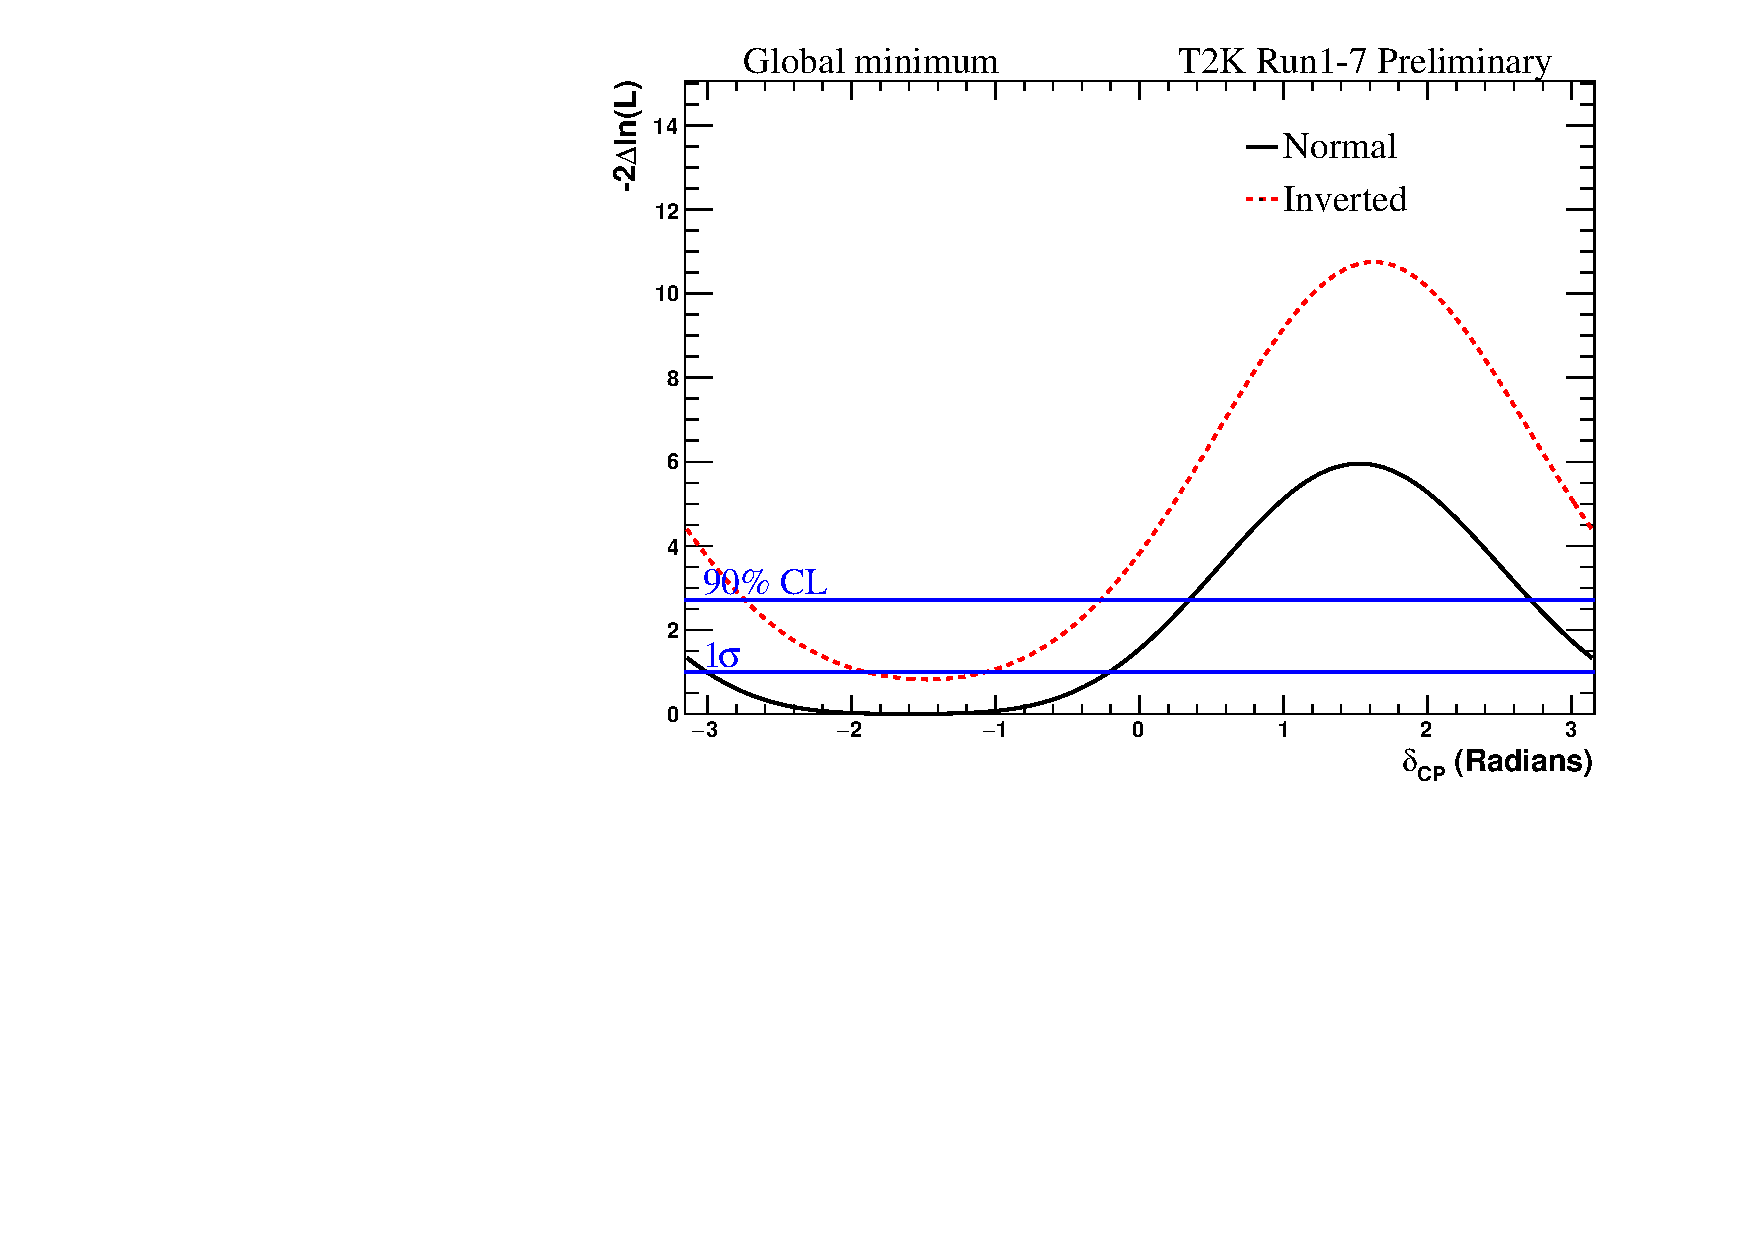
\includegraphics[trim={0cm 0cm 0cm 0cm}, clip, scale=0.33] {images/sensitivity/dcp_global_t2k}
				\caption*{without reactor constraint}
			\end{figure}
		\end{column}
		\begin{column}{0.5\paperwidth}
			\begin{figure}
				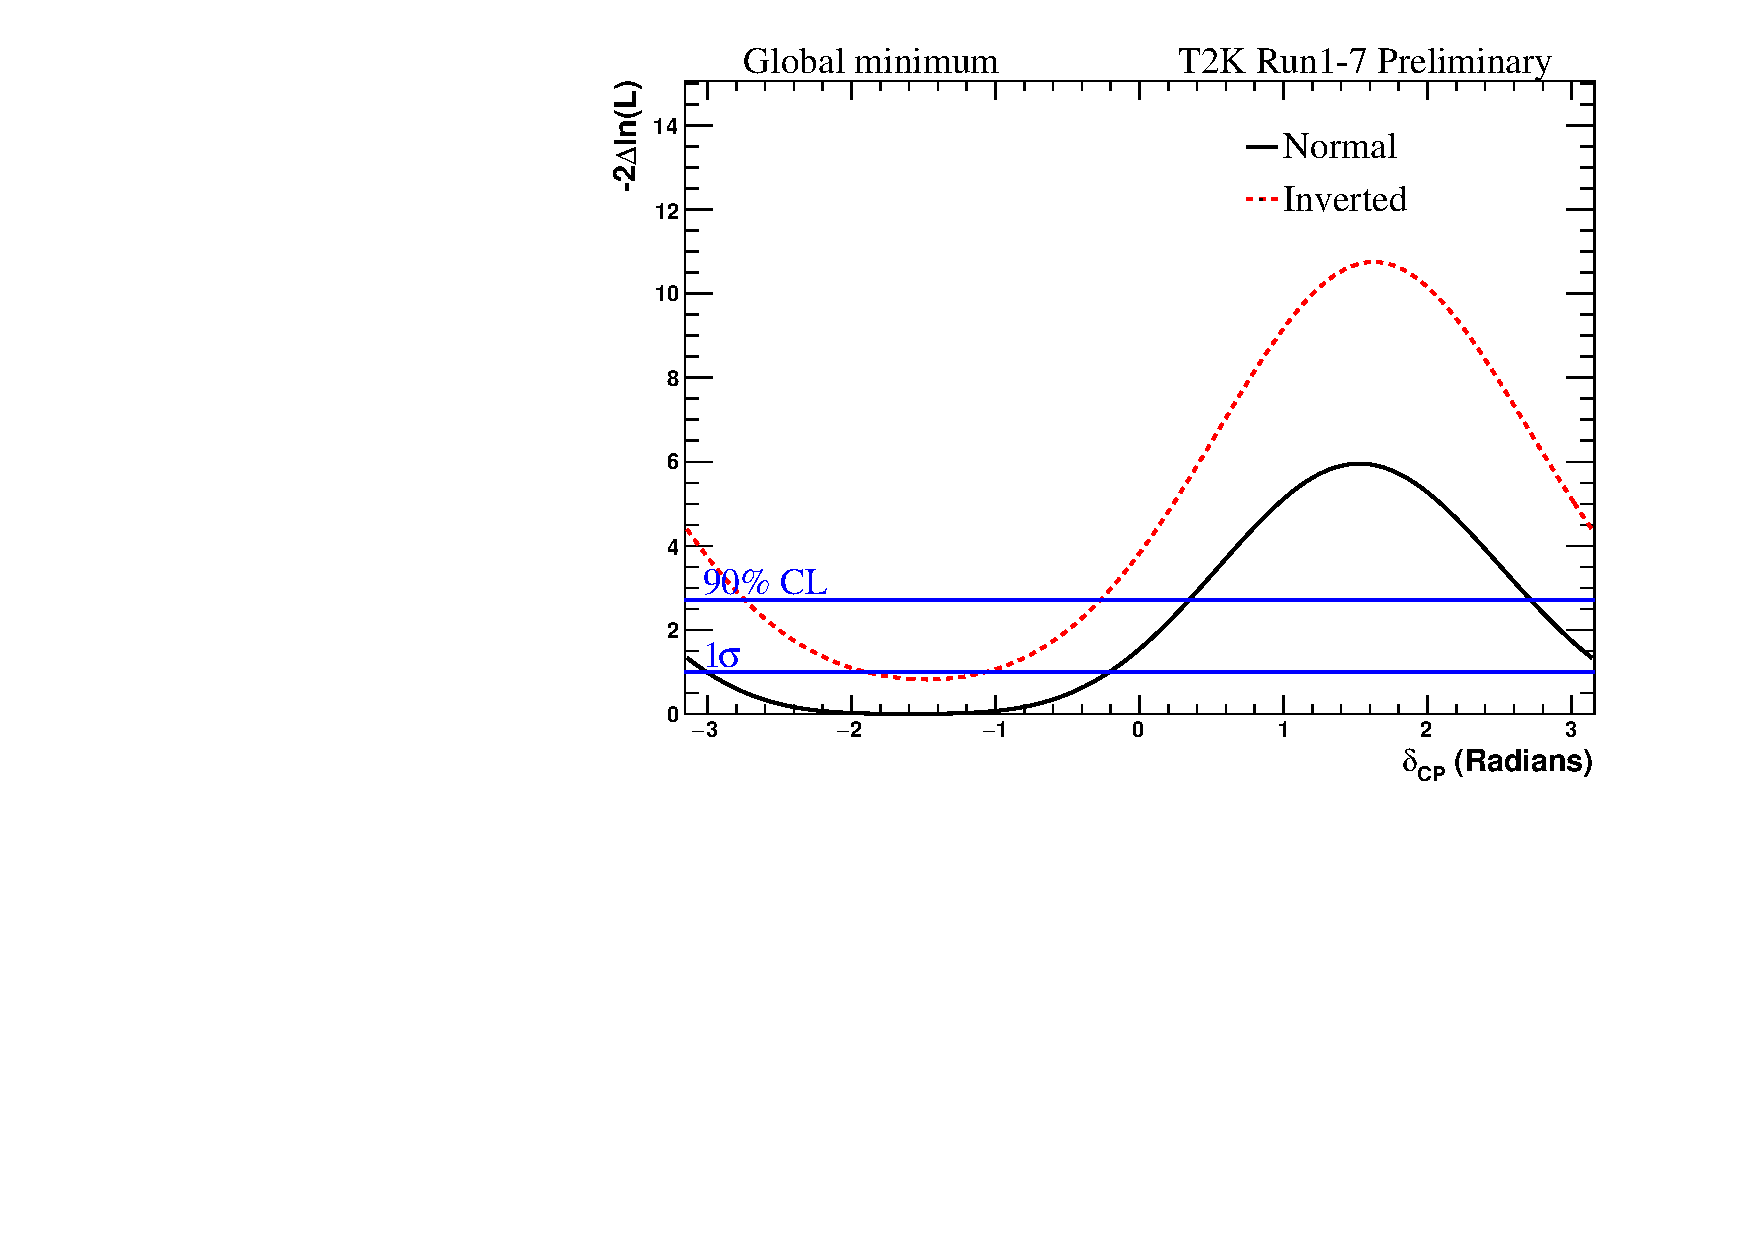
\includegraphics[trim={0cm 0cm 0cm 0cm}, clip, scale=0.33] {images/sensitivity/dcp_global_t2k}
				\caption*{with reactor constraint}
			\end{figure}
		\end{column}
	\end{columns}
\end{frame}

\begin{frame}{\deltacp sensitivity - Asimov B}
	\centering
	\begin{columns}
		\begin{column}{0.5\paperwidth}
			\begin{figure}
				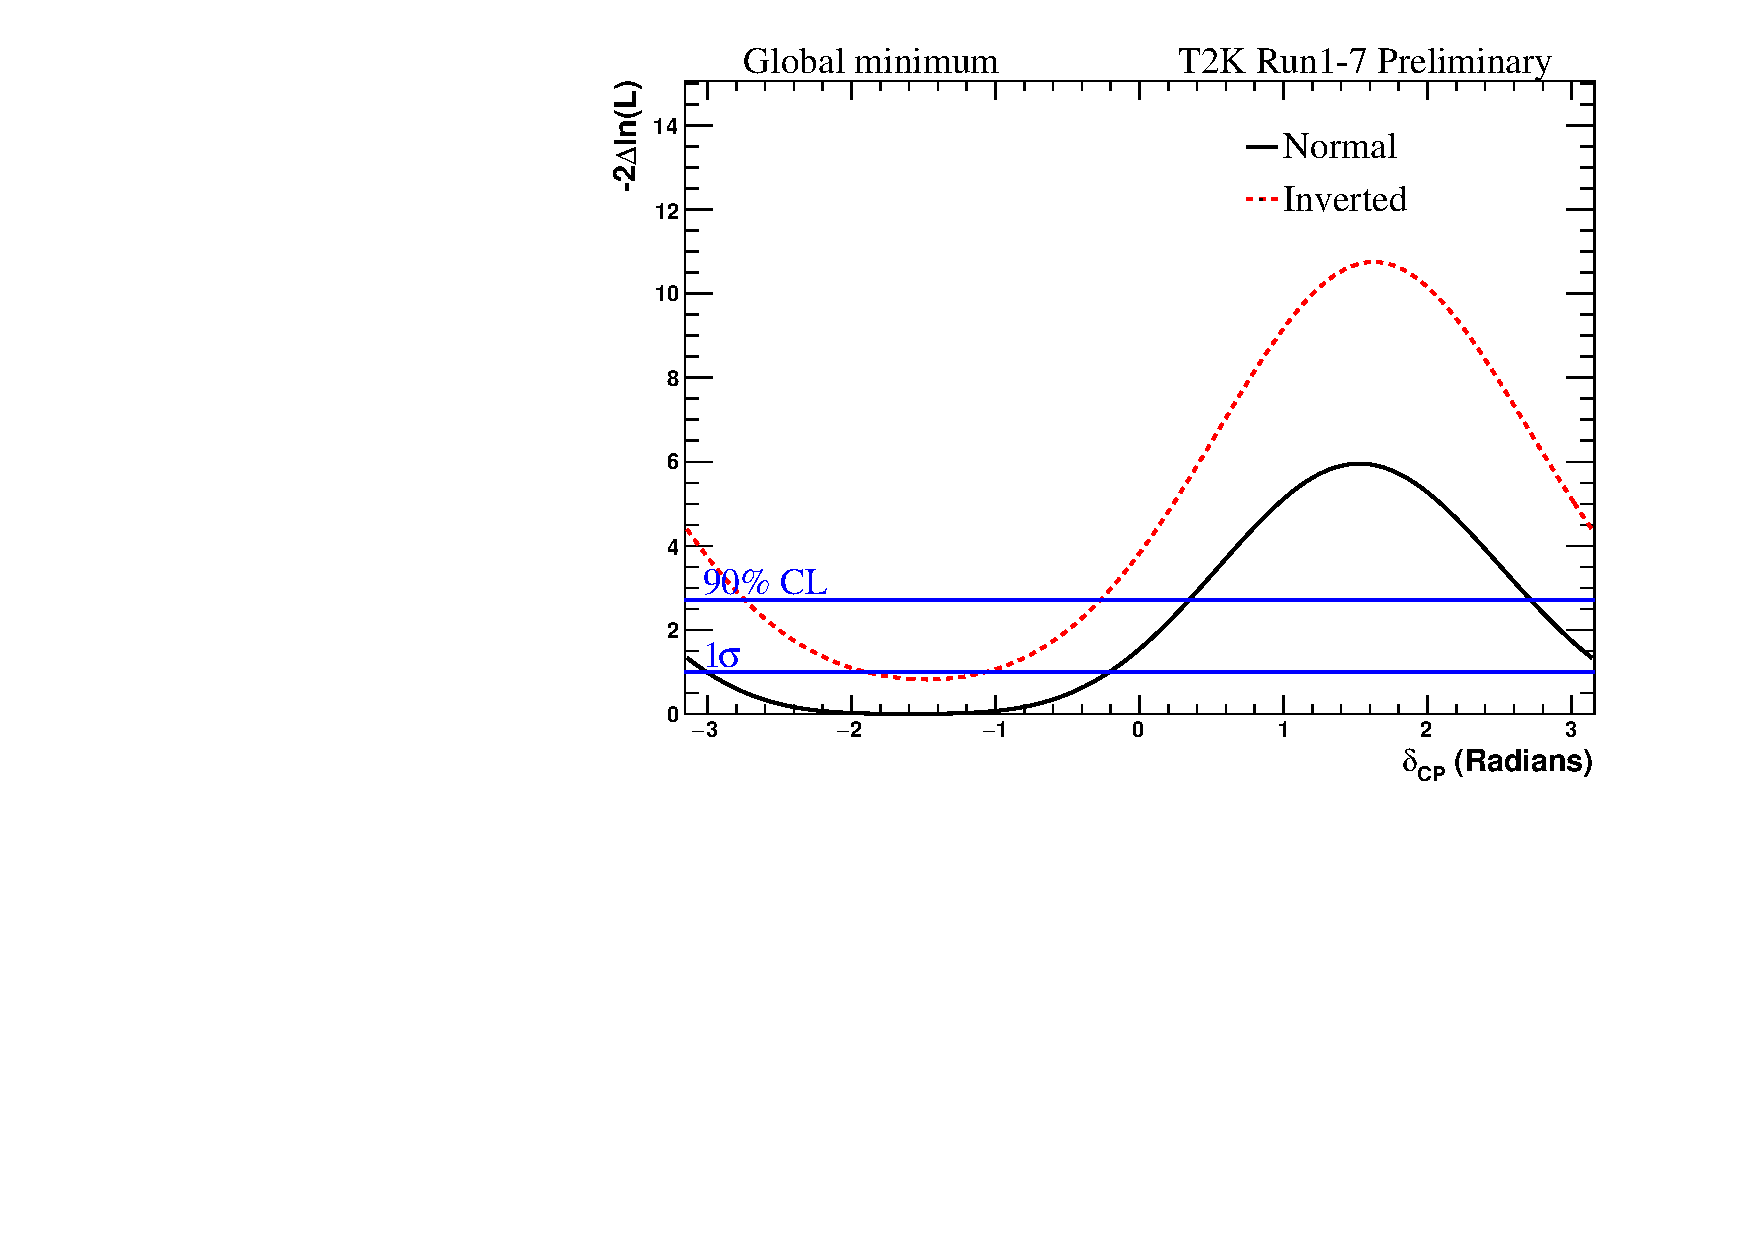
\includegraphics[trim={0cm 0cm 0cm 0cm}, clip, scale=0.33] {images/sensitivity/dcp_global_t2k}
				\caption*{without reactor constraint}
			\end{figure}
		\end{column}
		\begin{column}{0.5\paperwidth}
			\begin{figure}
				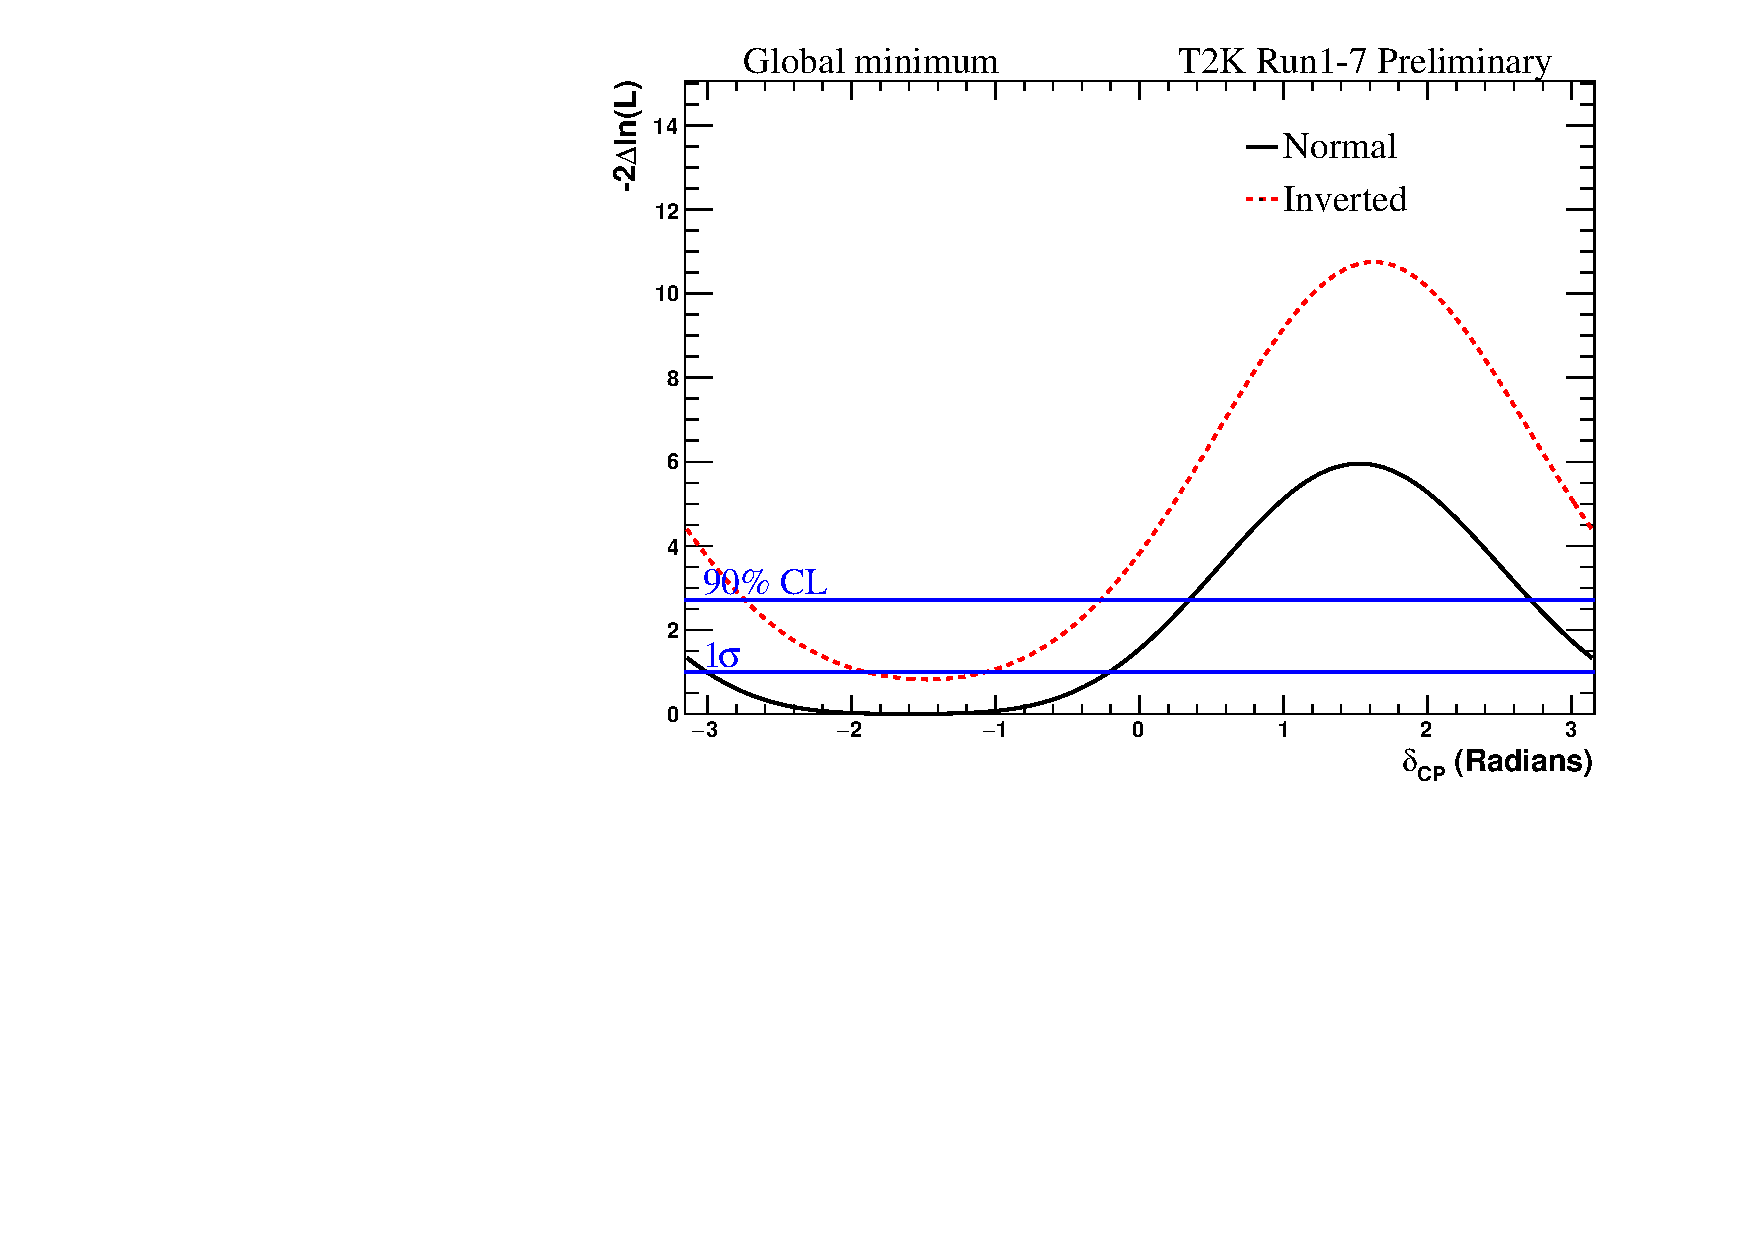
\includegraphics[trim={0cm 0cm 0cm 0cm}, clip, scale=0.33] {images/sensitivity/dcp_global_t2k}
				\caption*{with reactor constraint}
			\end{figure}
		\end{column}
	\end{columns}
\end{frame}

%===============================================================================
\section{\sinsqthetaonethree sensitivity}
\begin{frame}
	\centering
	\Large Run 1-8 \sinsqthetaonethree sensitivity\\
\end{frame}

\begin{frame}{\sinsqthetaonethree sensitivity - Asimov A}
	\centering
	\begin{columns}
		\begin{column}{0.5\paperwidth}
			\begin{figure}
				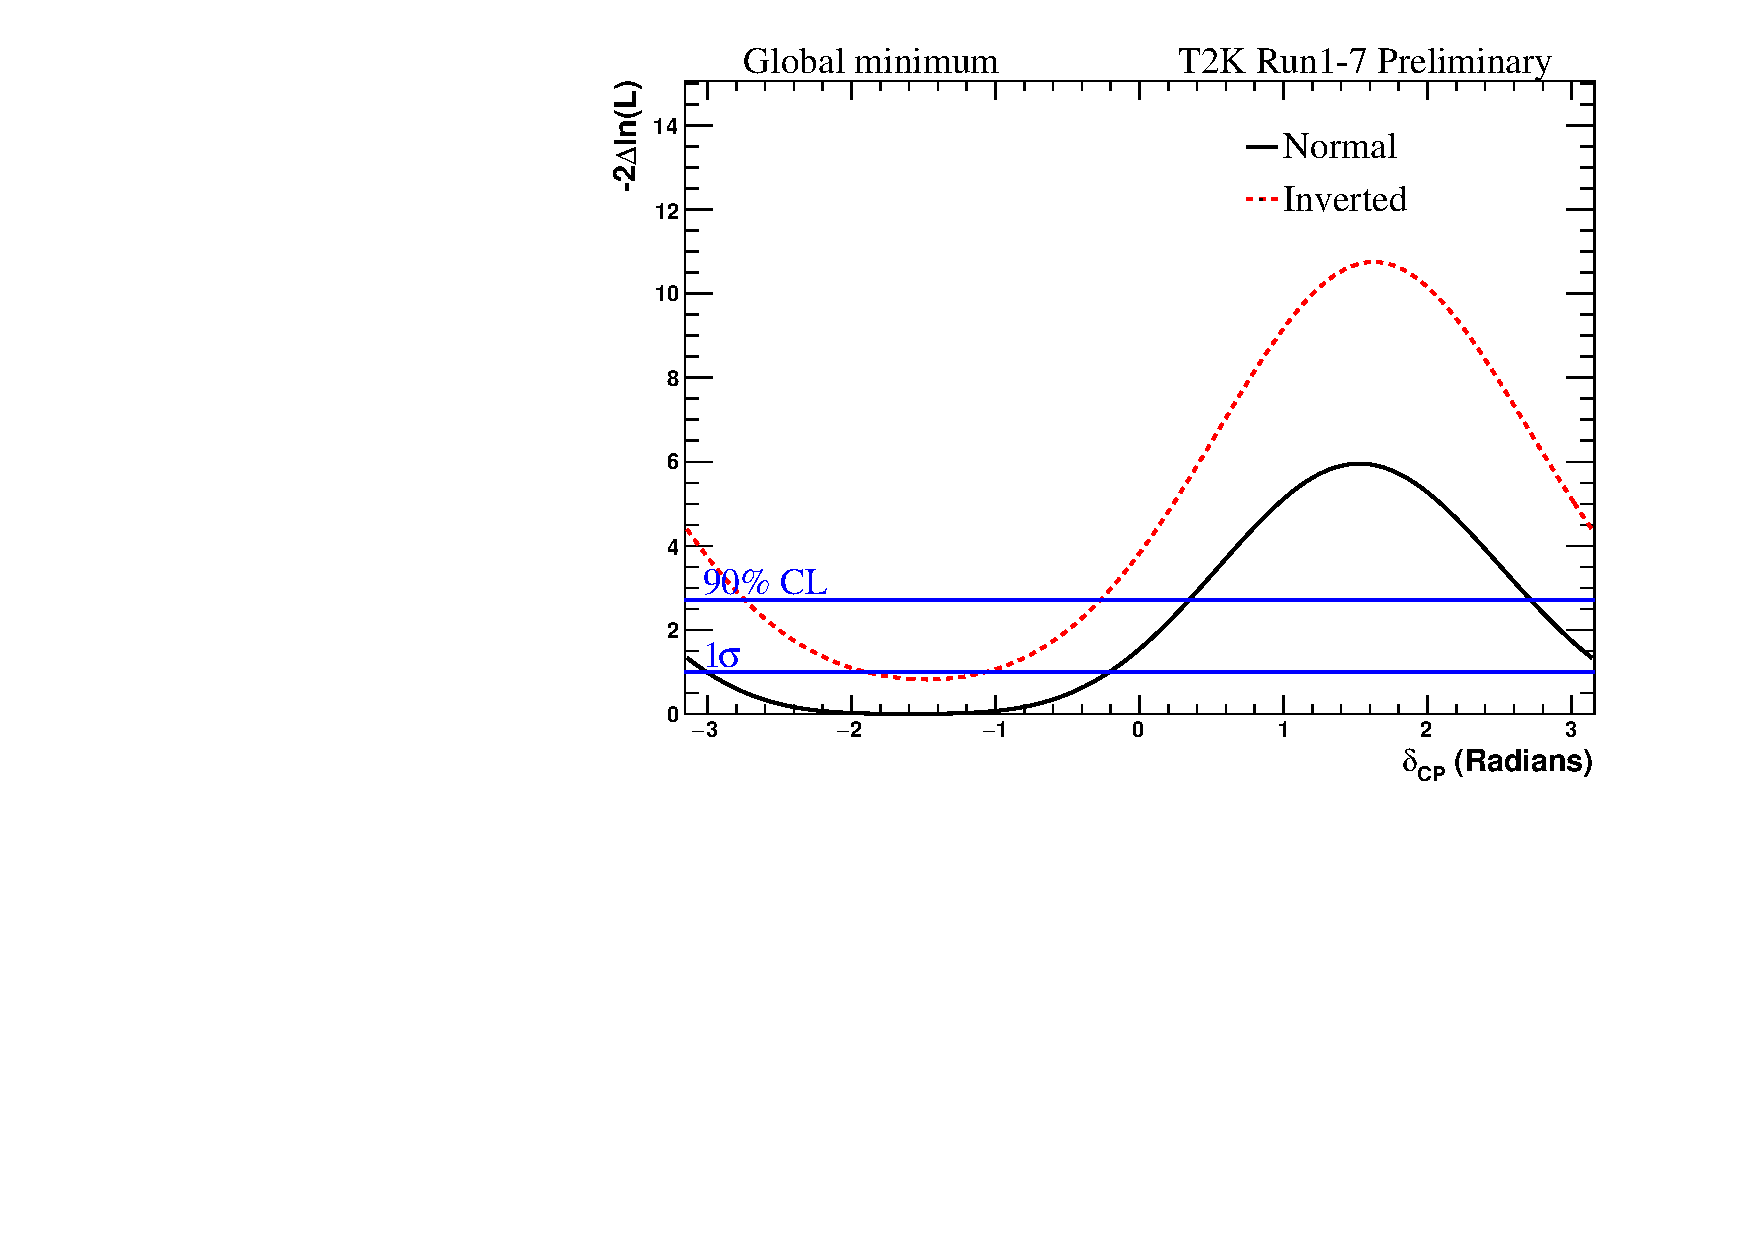
\includegraphics[trim={0cm 0cm 0cm 0cm}, clip, scale=0.33] {images/sensitivity/th13_global_t2k}
				\caption*{without reactor constraint}
			\end{figure}
		\end{column}
		\begin{column}{0.5\paperwidth}
			\begin{figure}
				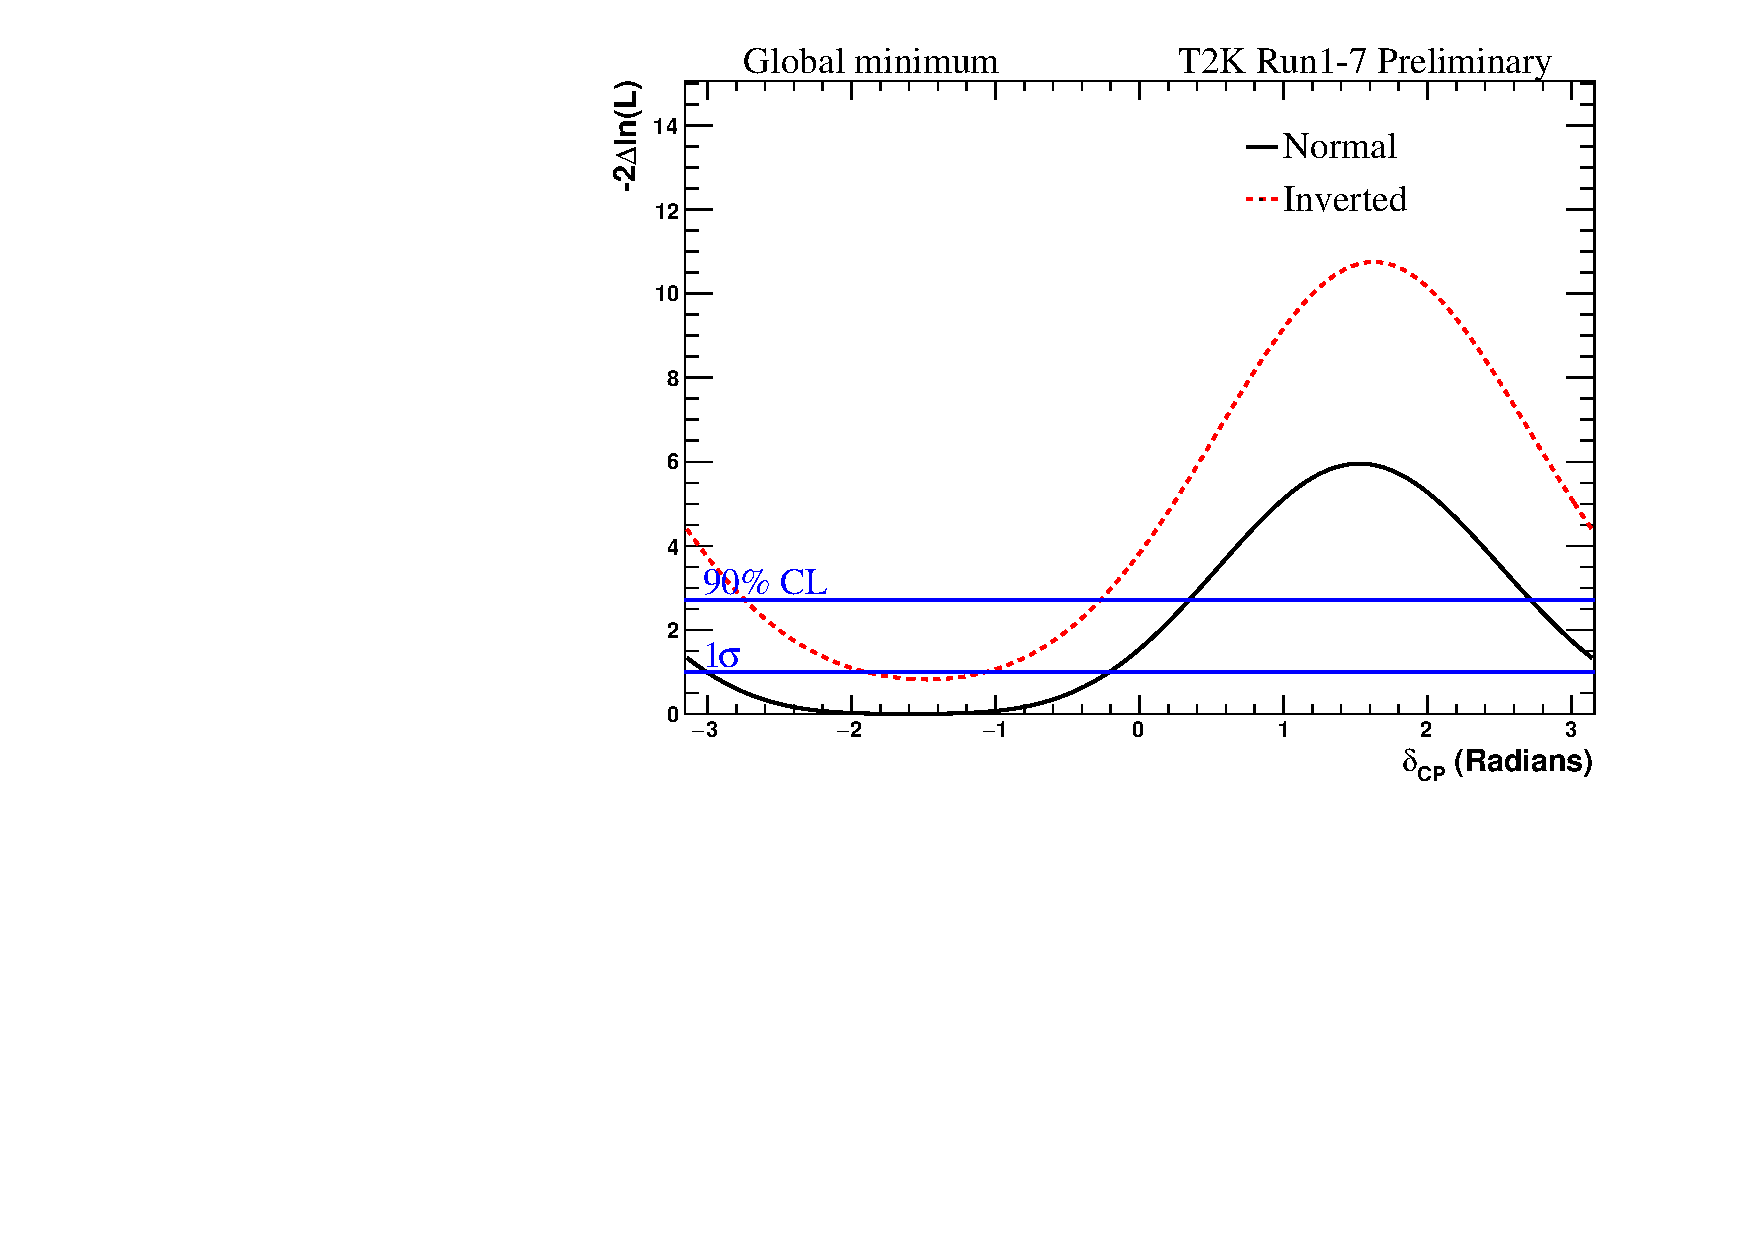
\includegraphics[trim={0cm 0cm 0cm 0cm}, clip, scale=0.33] {images/sensitivity/th13_global_t2k}
				\caption*{with reactor constraint}
			\end{figure}
		\end{column}
	\end{columns}
\end{frame}

\begin{frame}{\sinsqthetaonethree sensitivity - Asimov B}
	\centering
	\begin{columns}
		\begin{column}{0.5\paperwidth}
			\begin{figure}
				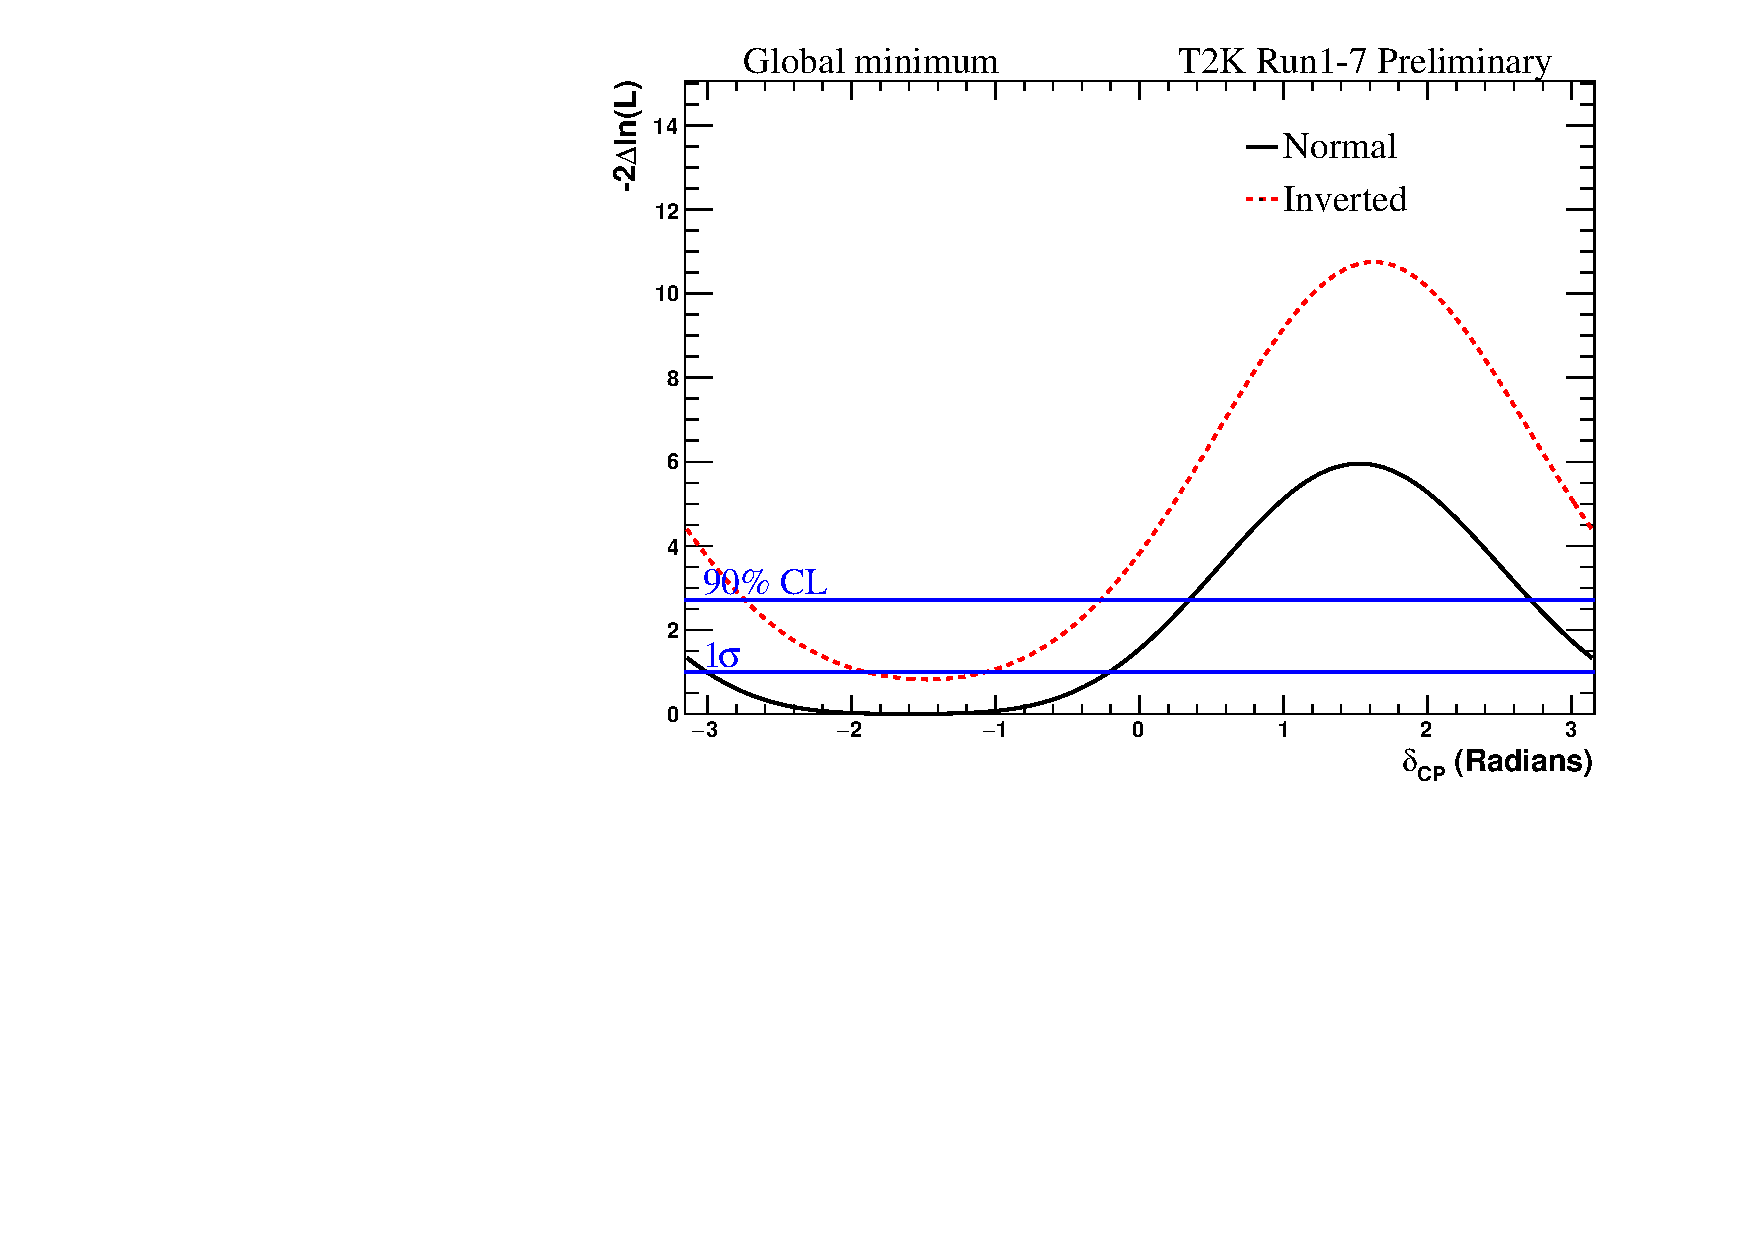
\includegraphics[trim={0cm 0cm 0cm 0cm}, clip, scale=0.33] {images/sensitivity/th13_global_t2k}
				\caption*{without reactor constraint}
			\end{figure}
		\end{column}
		\begin{column}{0.5\paperwidth}
			\begin{figure}
				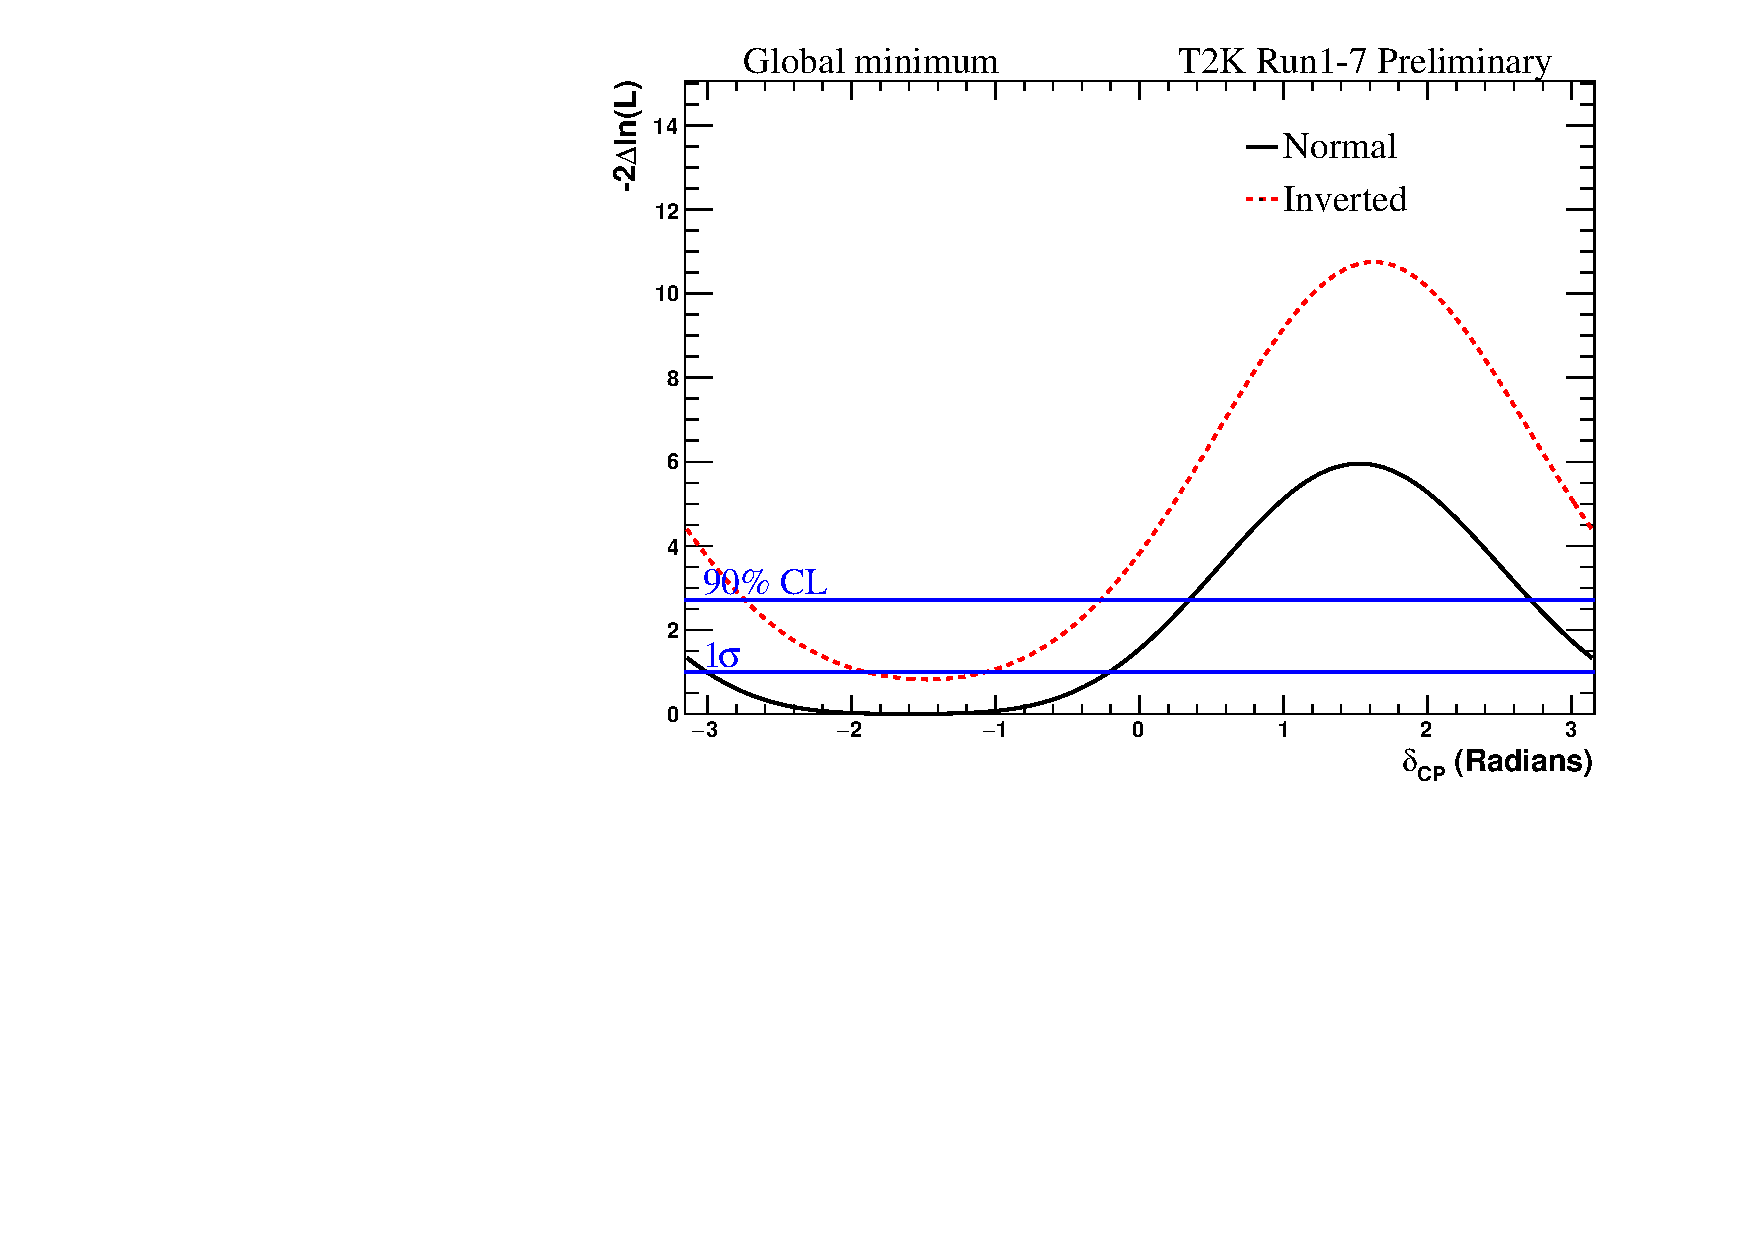
\includegraphics[trim={0cm 0cm 0cm 0cm}, clip, scale=0.33] {images/sensitivity/th13_global_t2k}
				\caption*{with reactor constraint}
			\end{figure}
		\end{column}
	\end{columns}
\end{frame}

%===============================================================================
\section{\sinsqthetatwothree sensitivity}
\begin{frame}
	\centering
	\Large Run 1-8 \sinsqthetatwothree sensitivity\\
\end{frame}

\begin{frame}{\sinsqthetatwothree sensitivity - Asimov A}
	\centering
	\begin{columns}
		\begin{column}{0.5\paperwidth}
			\begin{figure}
				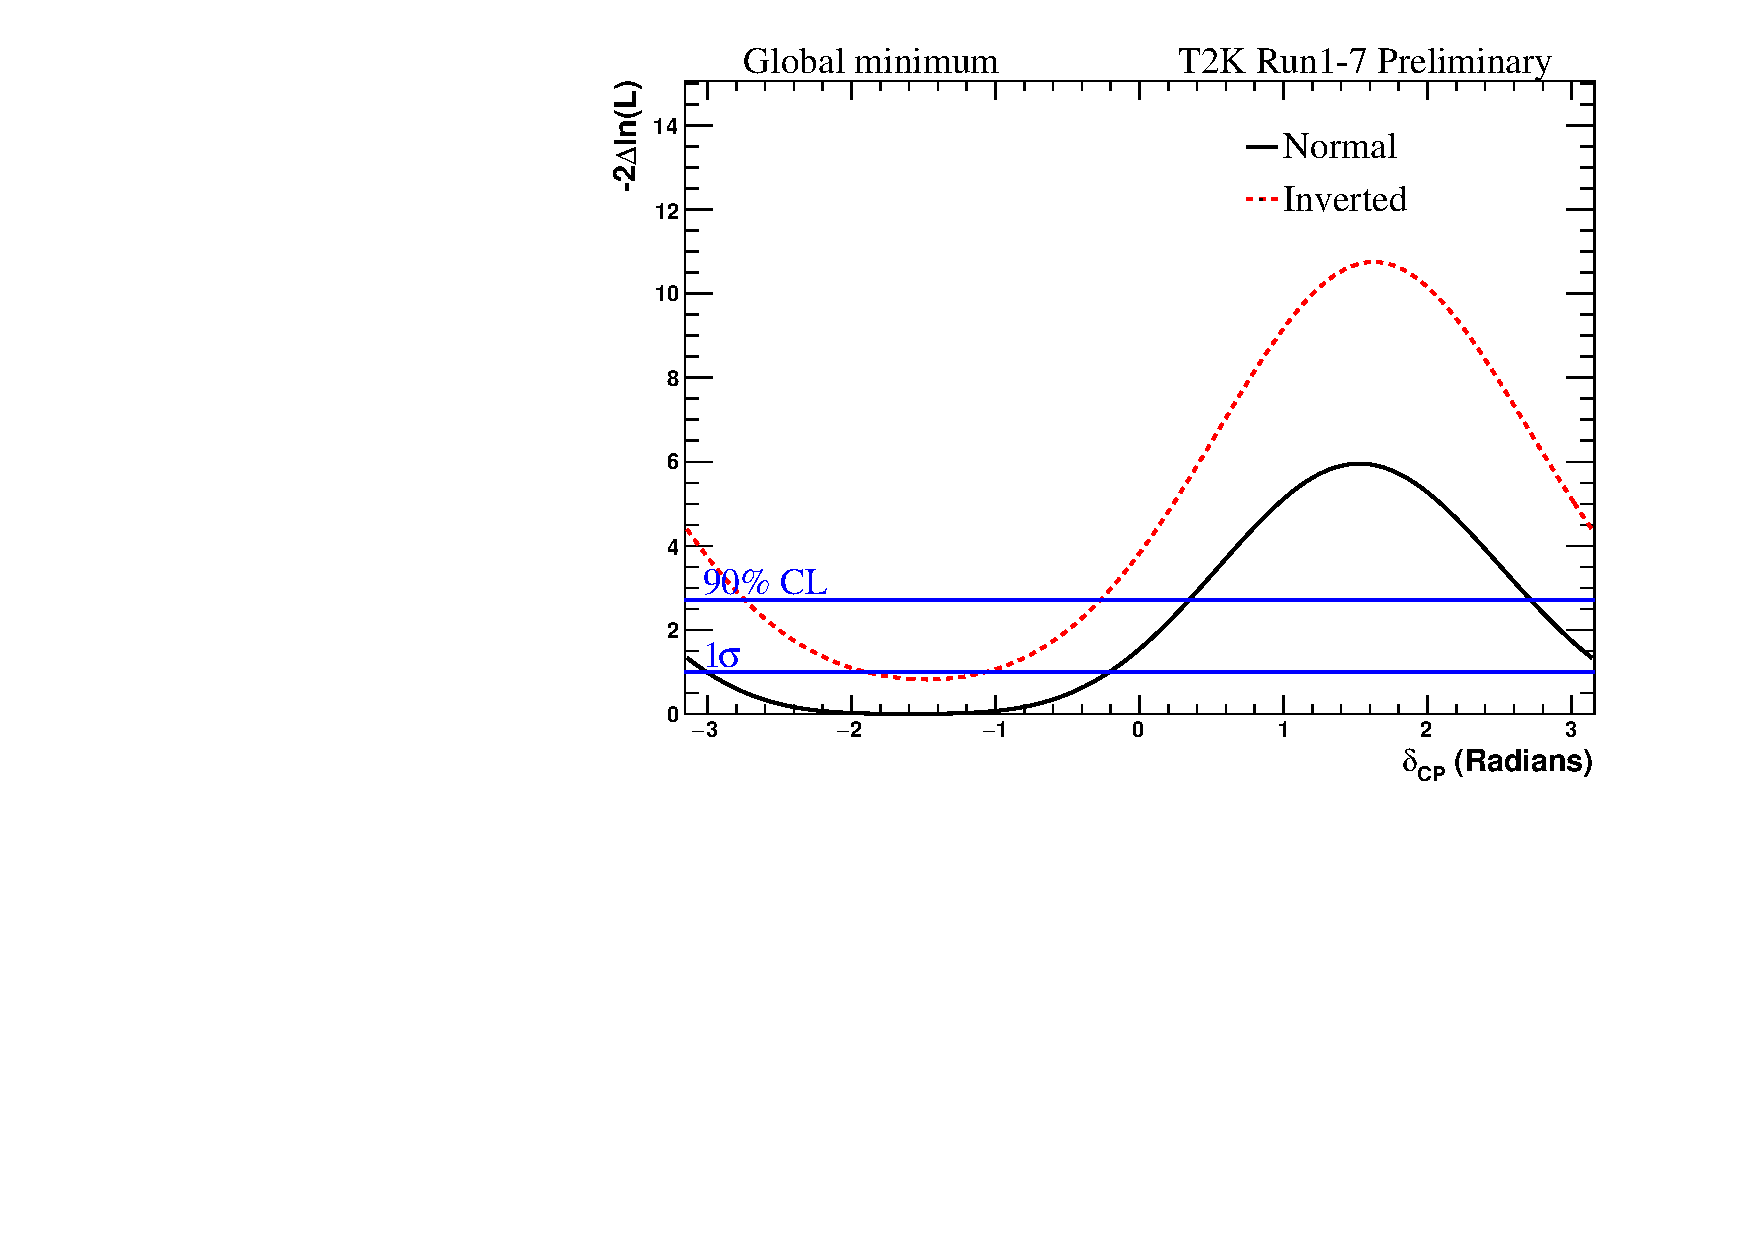
\includegraphics[trim={0cm 0cm 0cm 0cm}, clip, scale=0.33] {images/sensitivity/th23_global_t2k}
				\caption*{without reactor constraint}
			\end{figure}
		\end{column}
		\begin{column}{0.5\paperwidth}
			\begin{figure}
				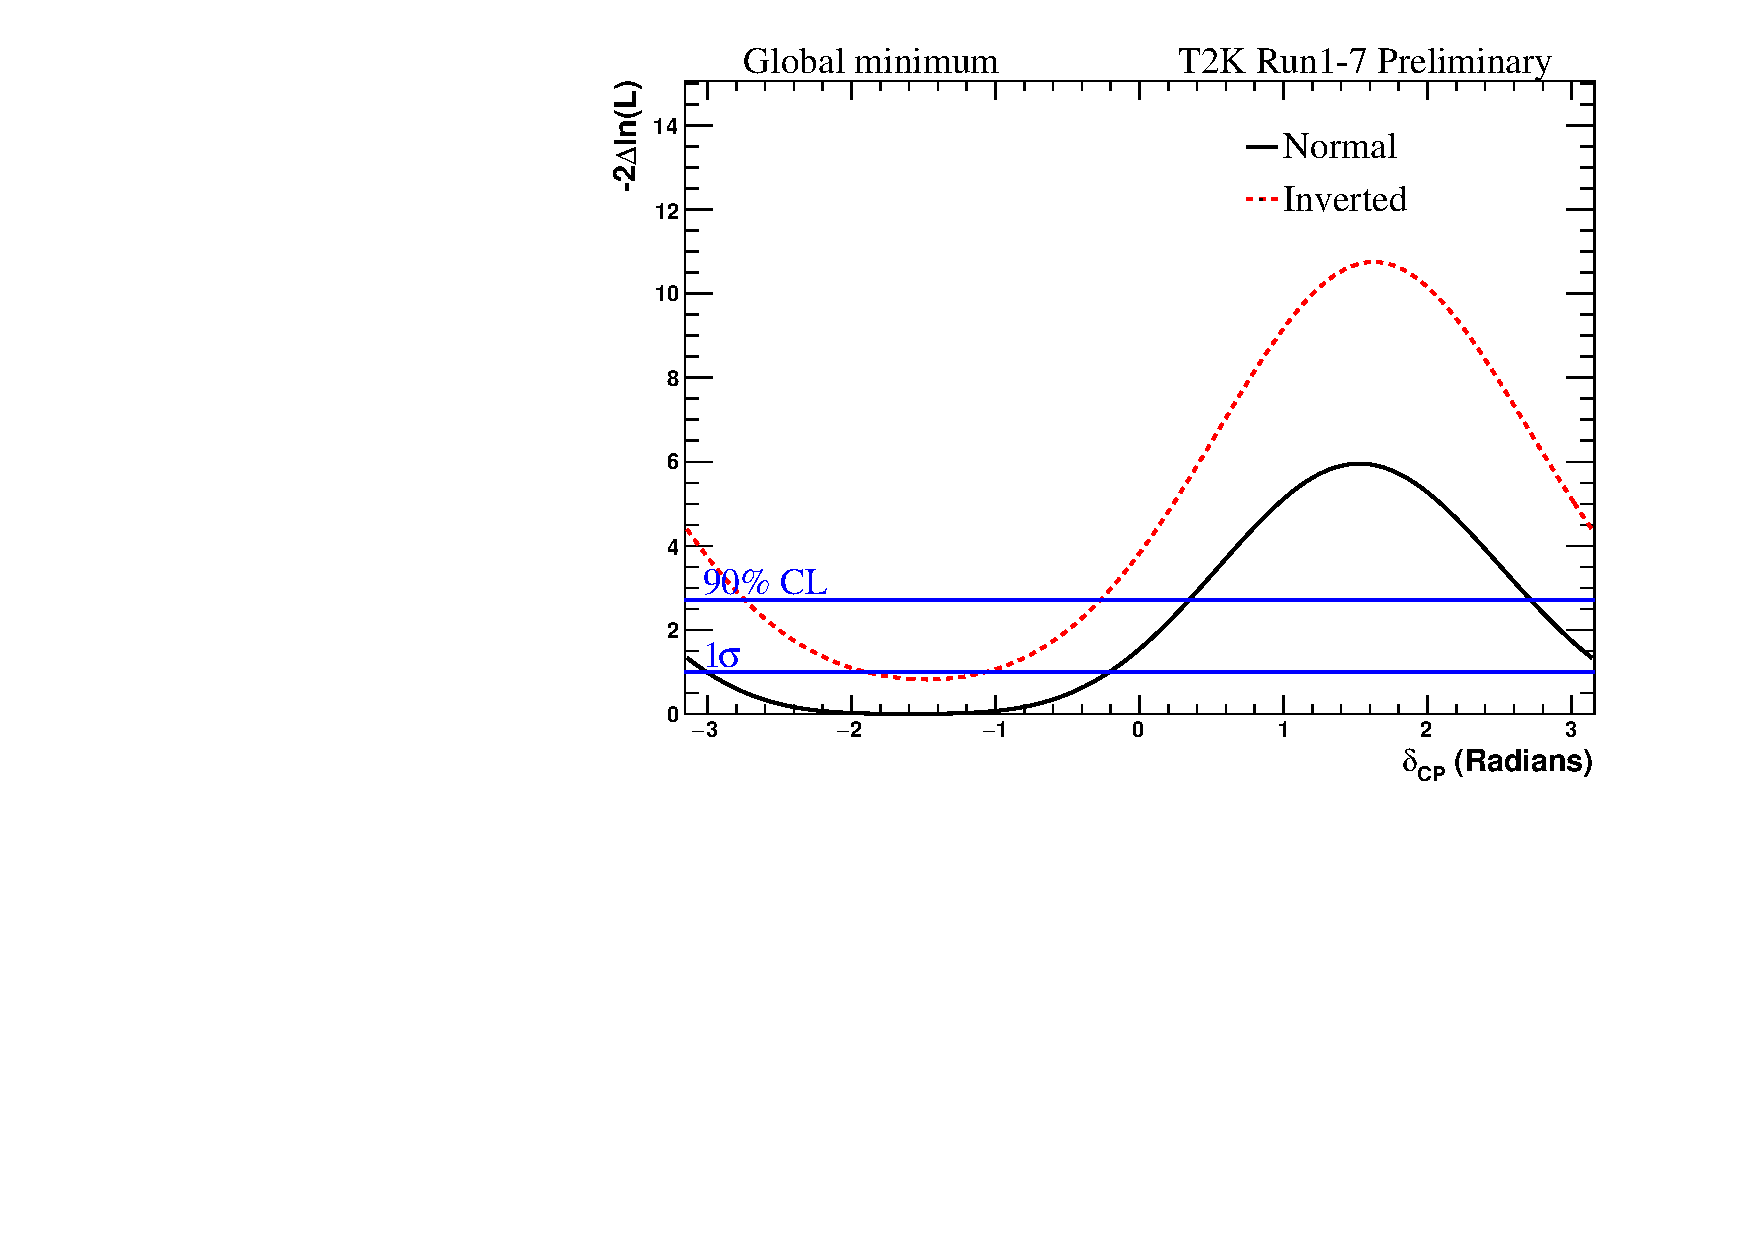
\includegraphics[trim={0cm 0cm 0cm 0cm}, clip, scale=0.33] {images/sensitivity/th23_global_t2k}
				\caption*{with reactor constraint}
			\end{figure}
		\end{column}
	\end{columns}
\end{frame}

\begin{frame}{\sinsqthetatwothree sensitivity - Asimov B}
	\centering
	\begin{columns}
		\begin{column}{0.5\paperwidth}
			\begin{figure}
				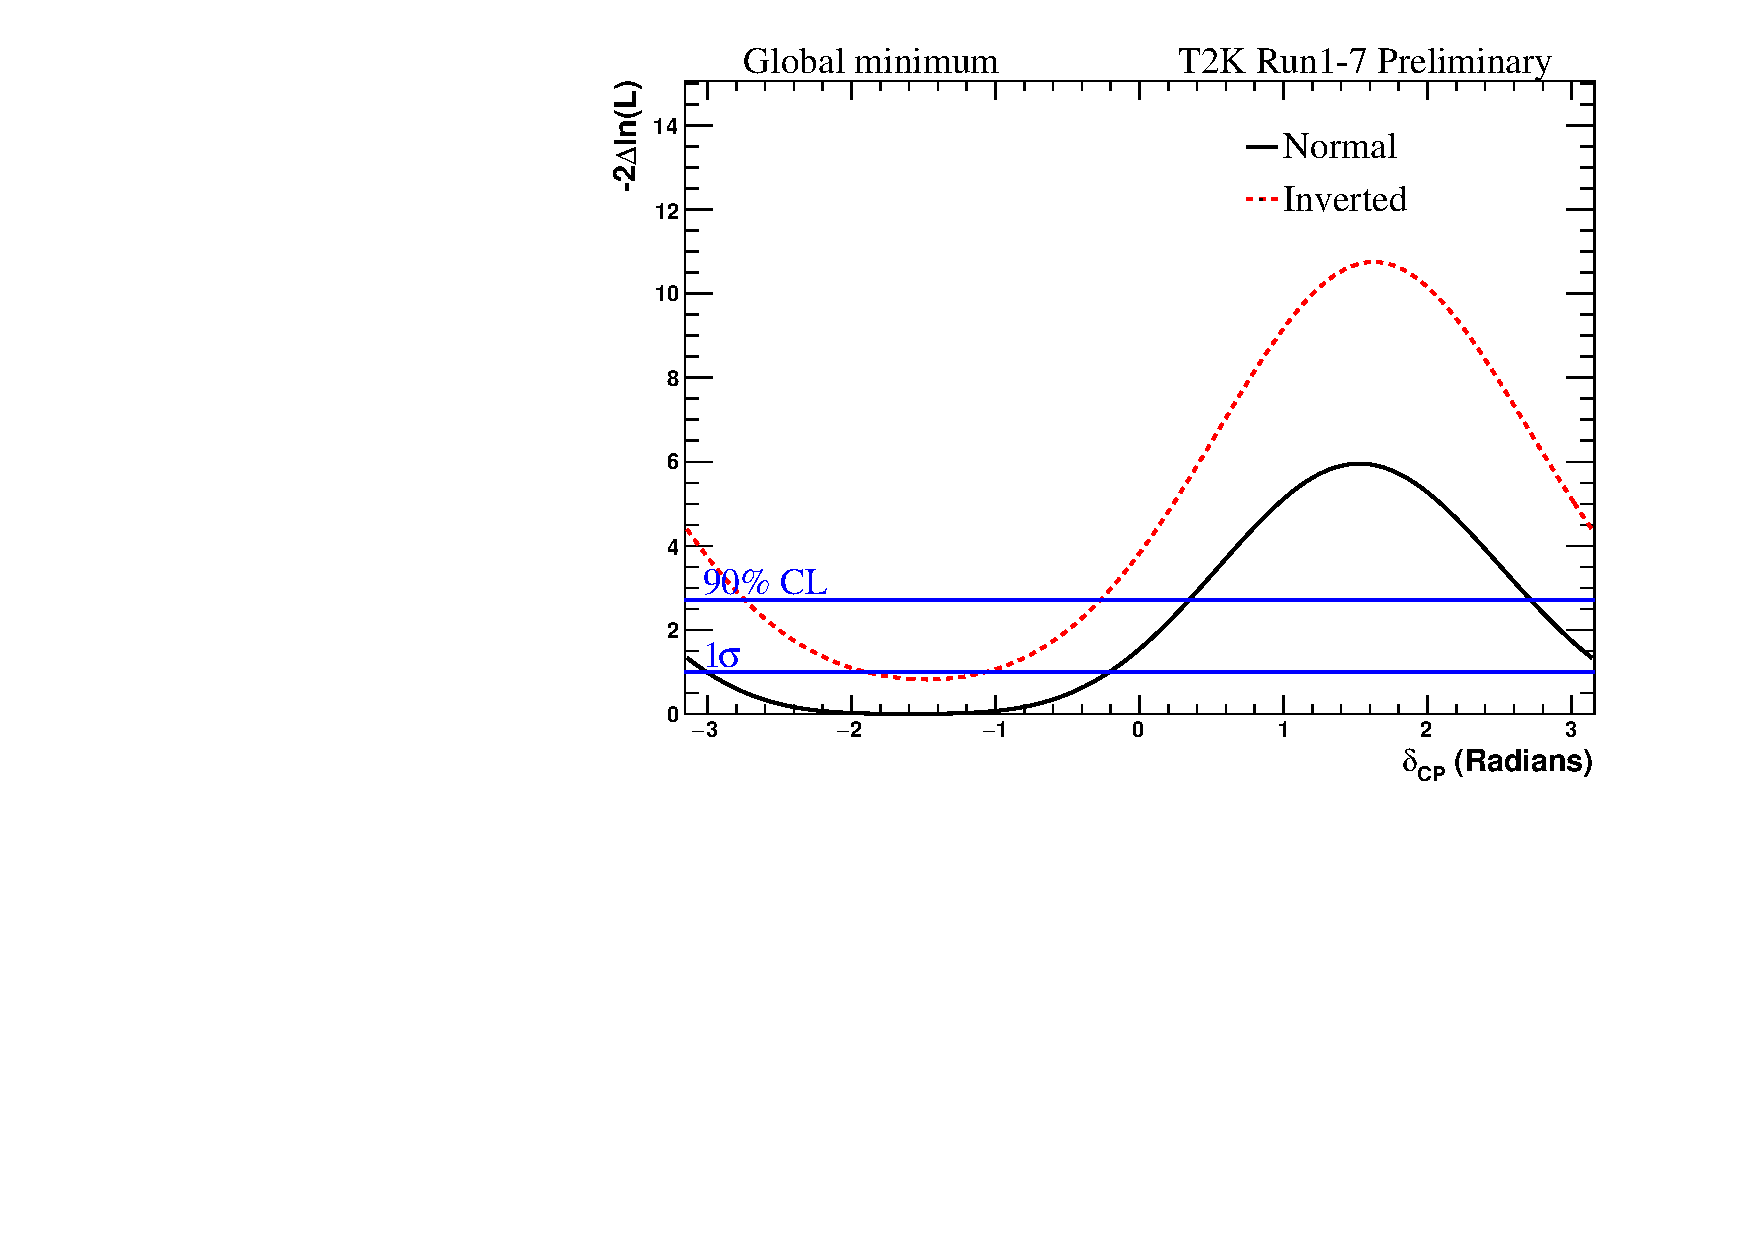
\includegraphics[trim={0cm 0cm 0cm 0cm}, clip, scale=0.33] {images/sensitivity/th23_global_t2k}
				\caption*{without reactor constraint}
			\end{figure}
		\end{column}
		\begin{column}{0.5\paperwidth}
			\begin{figure}
				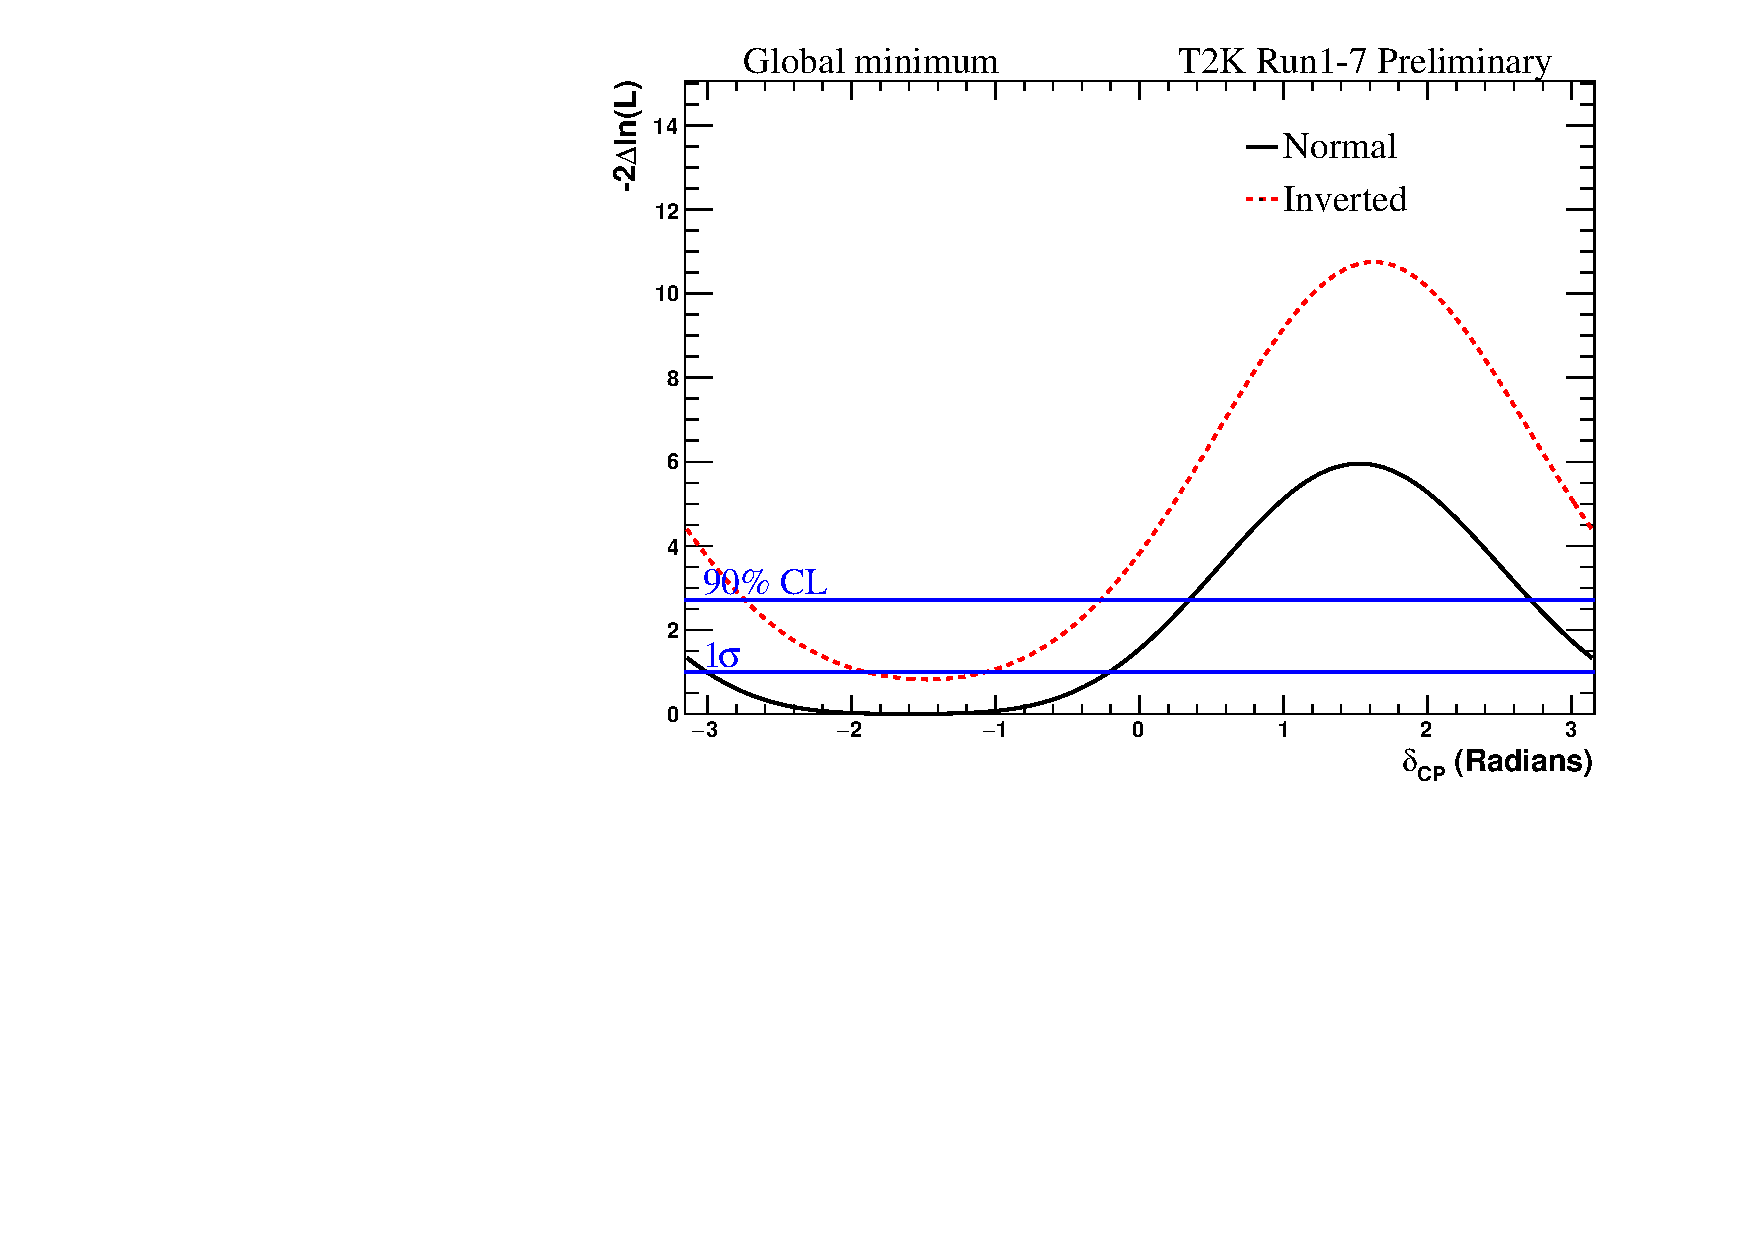
\includegraphics[trim={0cm 0cm 0cm 0cm}, clip, scale=0.33] {images/sensitivity/th23_global_t2k}
				\caption*{with reactor constraint}
			\end{figure}
		\end{column}
	\end{columns}
\end{frame}

%===============================================================================
\section{\dmsqtwothree sensitivity}
\begin{frame}
	\centering
	\Large Run 1-8 \dmsqtwothree sensitivity\\
\end{frame}

\begin{frame}{\dmsqtwothree sensitivity - Asimov A}
	\centering
	\begin{columns}
		\begin{column}{0.5\paperwidth}
			\begin{figure}
				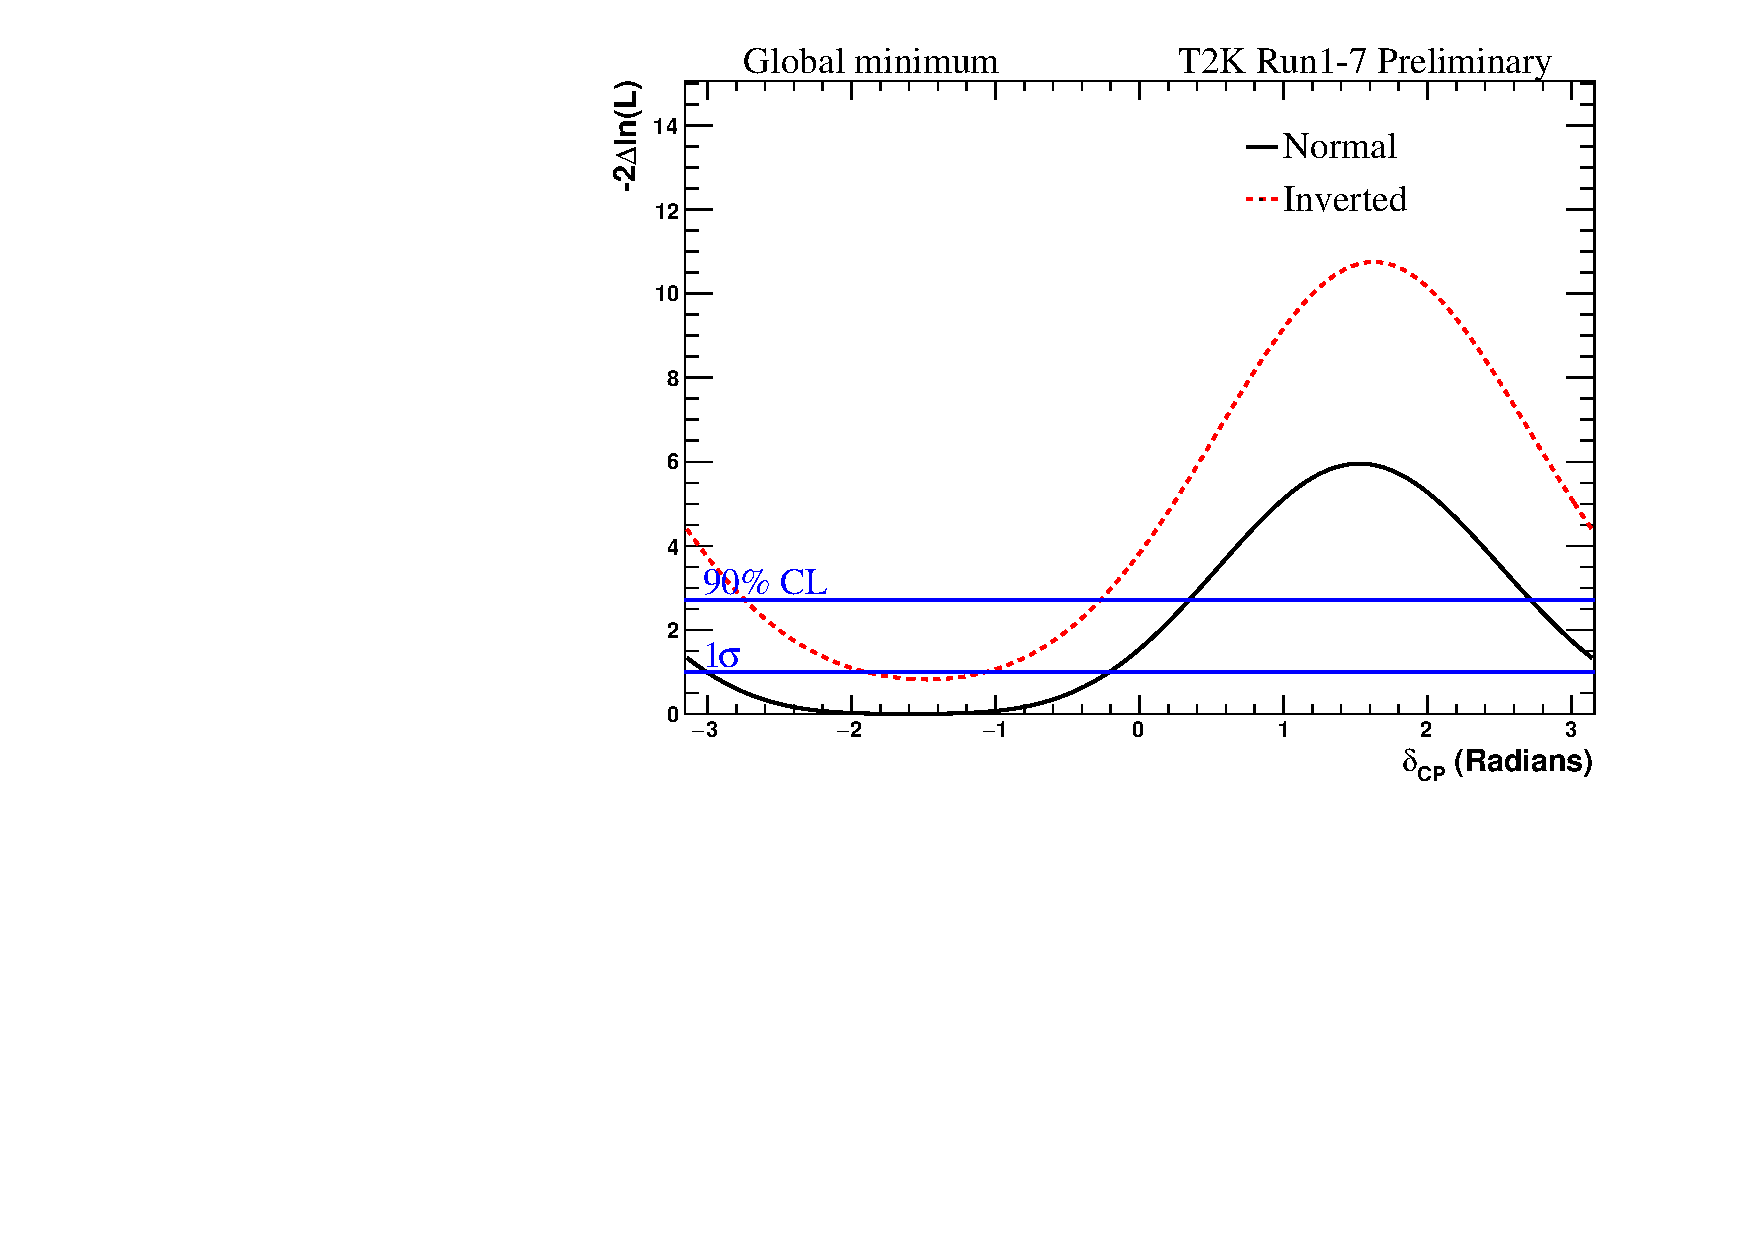
\includegraphics[trim={0cm 0cm 0cm 0cm}, clip, scale=0.33] {images/sensitivity/dmsq23_global_t2k}
				\caption*{without reactor constraint}
			\end{figure}
		\end{column}
		\begin{column}{0.5\paperwidth}
			\begin{figure}
				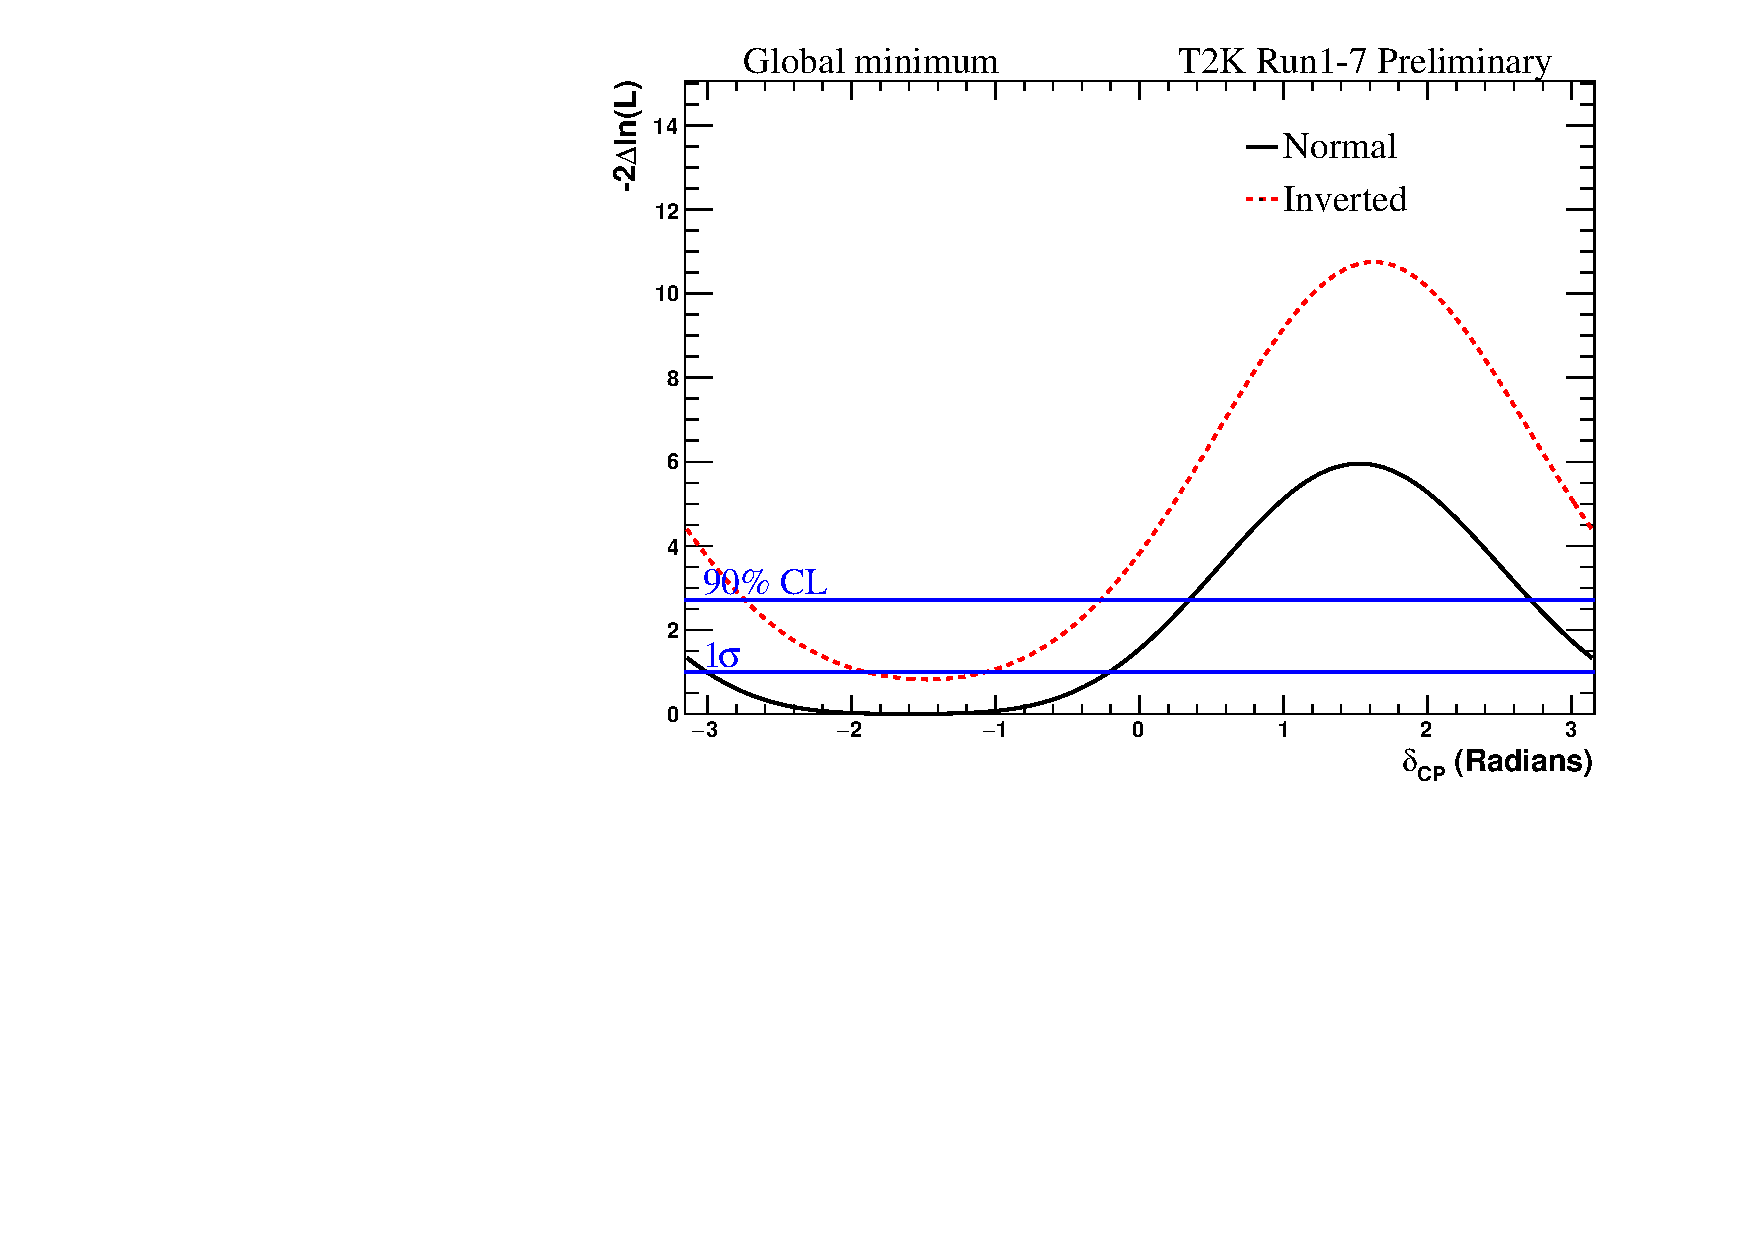
\includegraphics[trim={0cm 0cm 0cm 0cm}, clip, scale=0.33] {images/sensitivity/dmsq23_global_t2k}
				\caption*{with reactor constraint}
			\end{figure}
		\end{column}
	\end{columns}
\end{frame}

\begin{frame}{\dmsqtwothree sensitivity - Asimov B}
	\centering
	\begin{columns}
		\begin{column}{0.5\paperwidth}
			\begin{figure}
				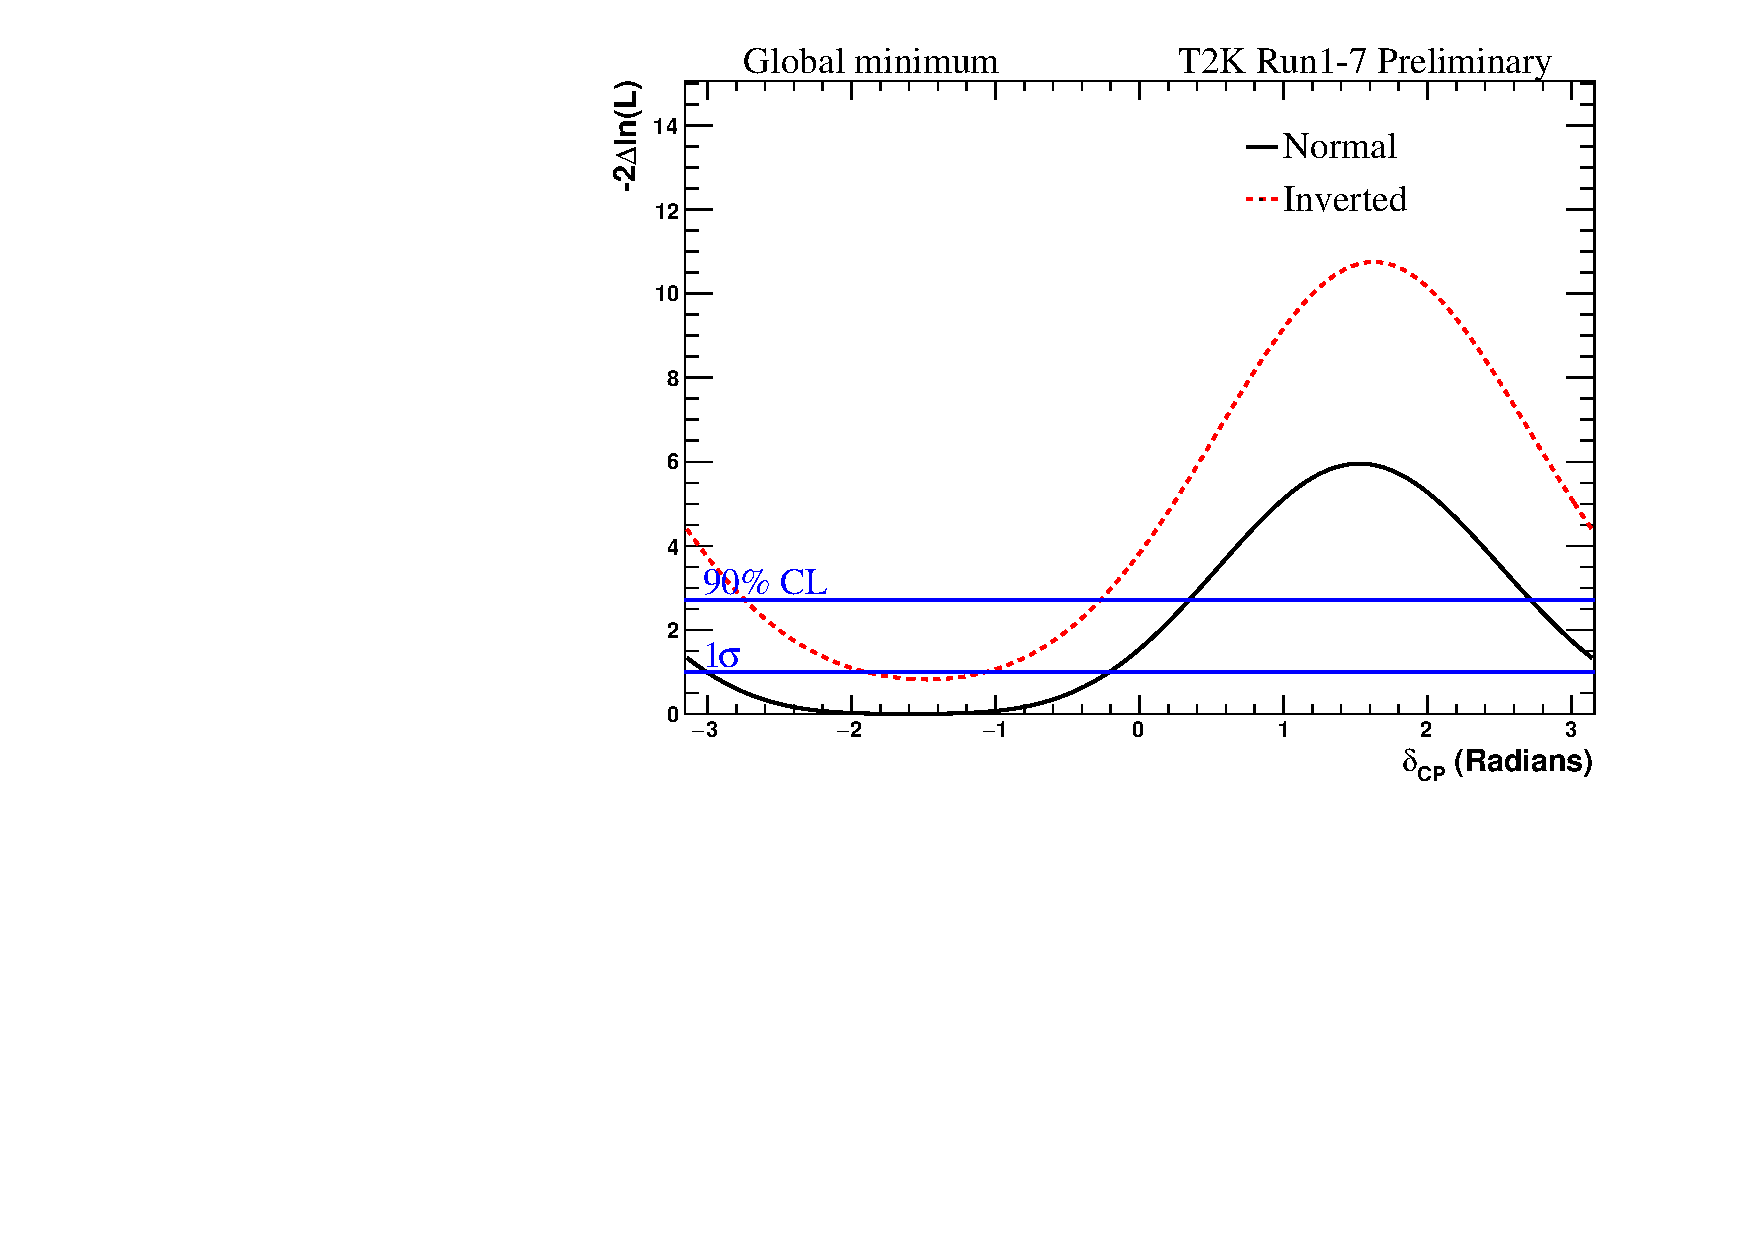
\includegraphics[trim={0cm 0cm 0cm 0cm}, clip, scale=0.33] {images/sensitivity/dmsq23_global_t2k}
				\caption*{without reactor constraint}
			\end{figure}
		\end{column}
		\begin{column}{0.5\paperwidth}
			\begin{figure}
				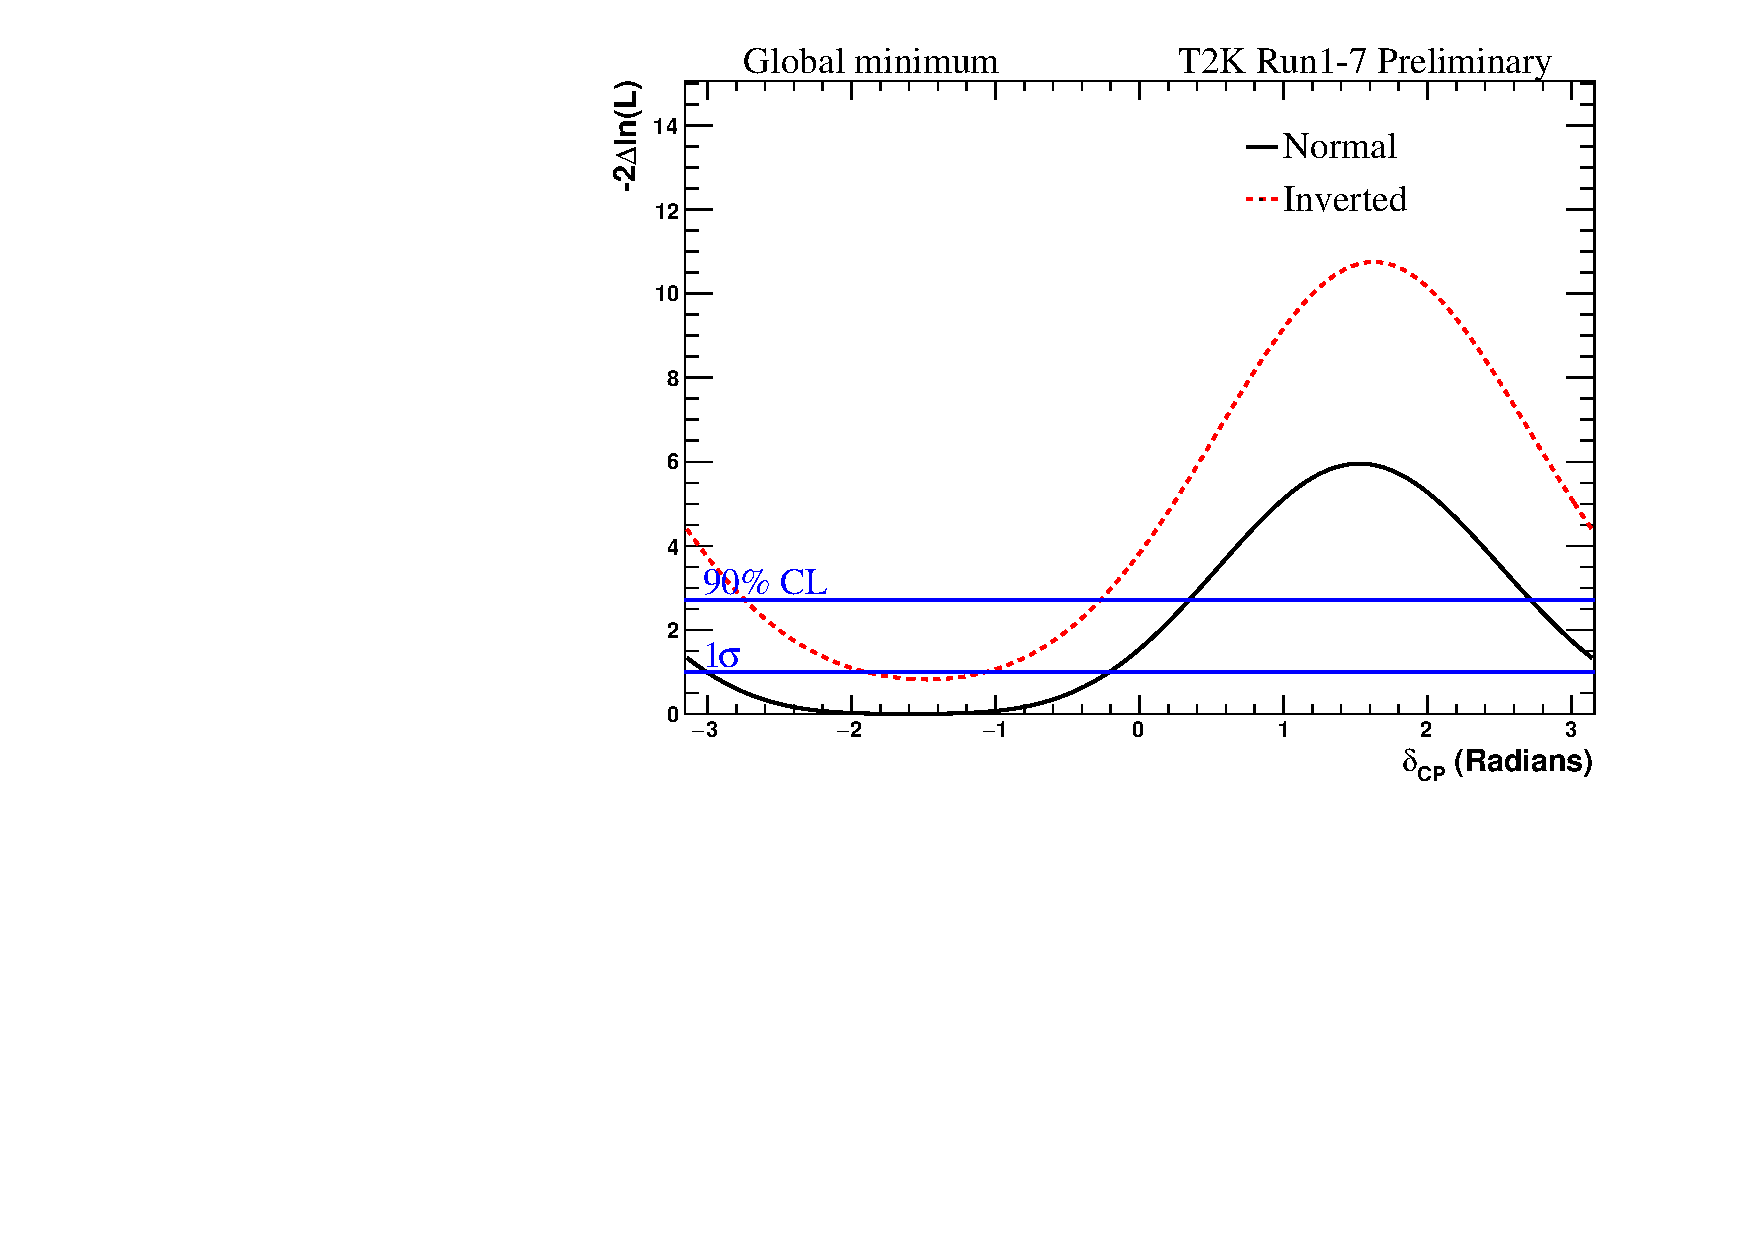
\includegraphics[trim={0cm 0cm 0cm 0cm}, clip, scale=0.33] {images/sensitivity/dmsq23_global_t2k}
				\caption*{with reactor constraint}
			\end{figure}
		\end{column}
	\end{columns}
\end{frame}

%===============================================================================
\section{\sinsqthetaonethree vs \deltacp sensitivity}
\begin{frame}
	\centering
	\Large Run 1-8 \sinsqthetaonethree vs \deltacp sensitivity\\
\end{frame}

\begin{frame}{\sinsqthetaonethree vs \deltacp sensitivity - Asimov A}
	\centering
	\begin{columns}
		\begin{column}{0.5\paperwidth}
			\begin{figure}
				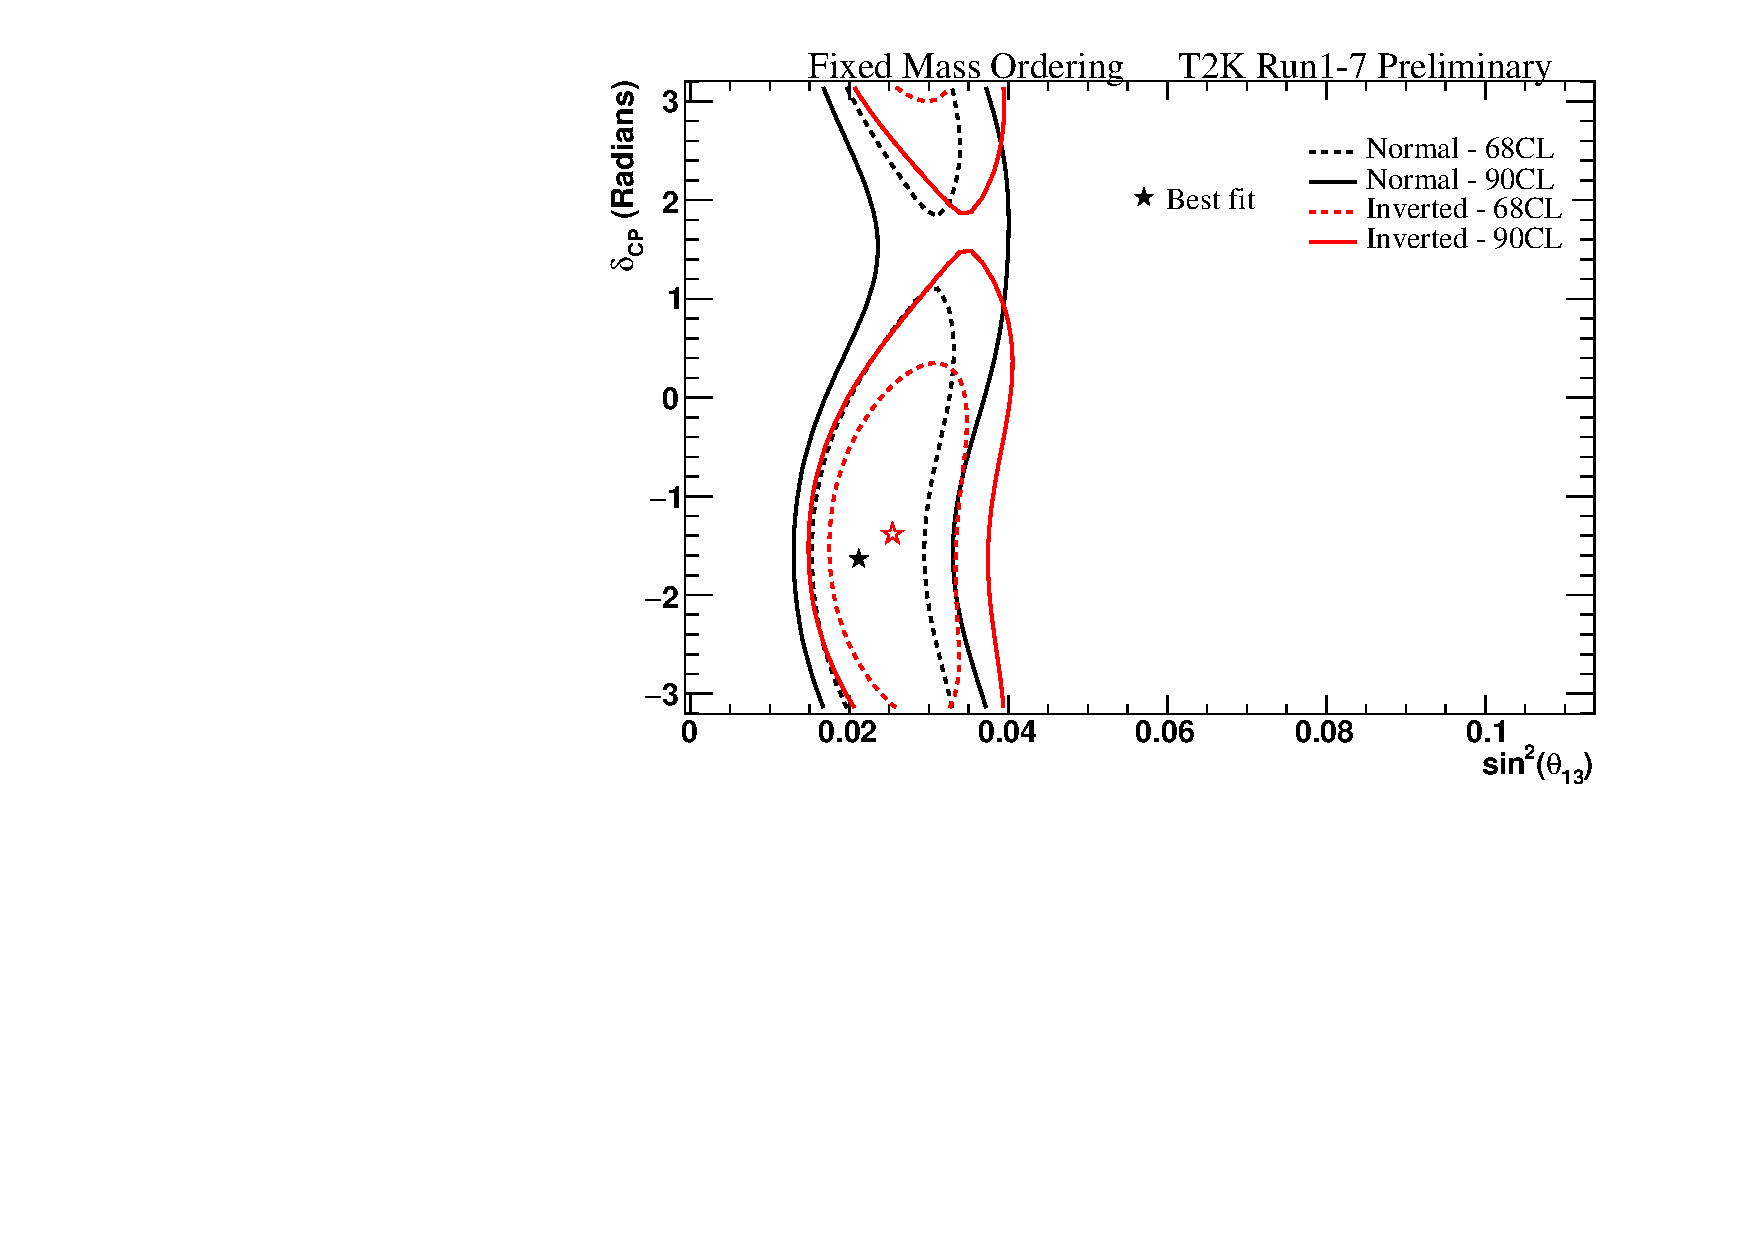
\includegraphics[trim={0cm 0cm 0cm 0cm}, clip, scale=0.33] {images/sensitivity/th13_dcp_global_t2k}
				\caption*{without reactor constraint}
			\end{figure}
		\end{column}
		\begin{column}{0.5\paperwidth}
			\begin{figure}
				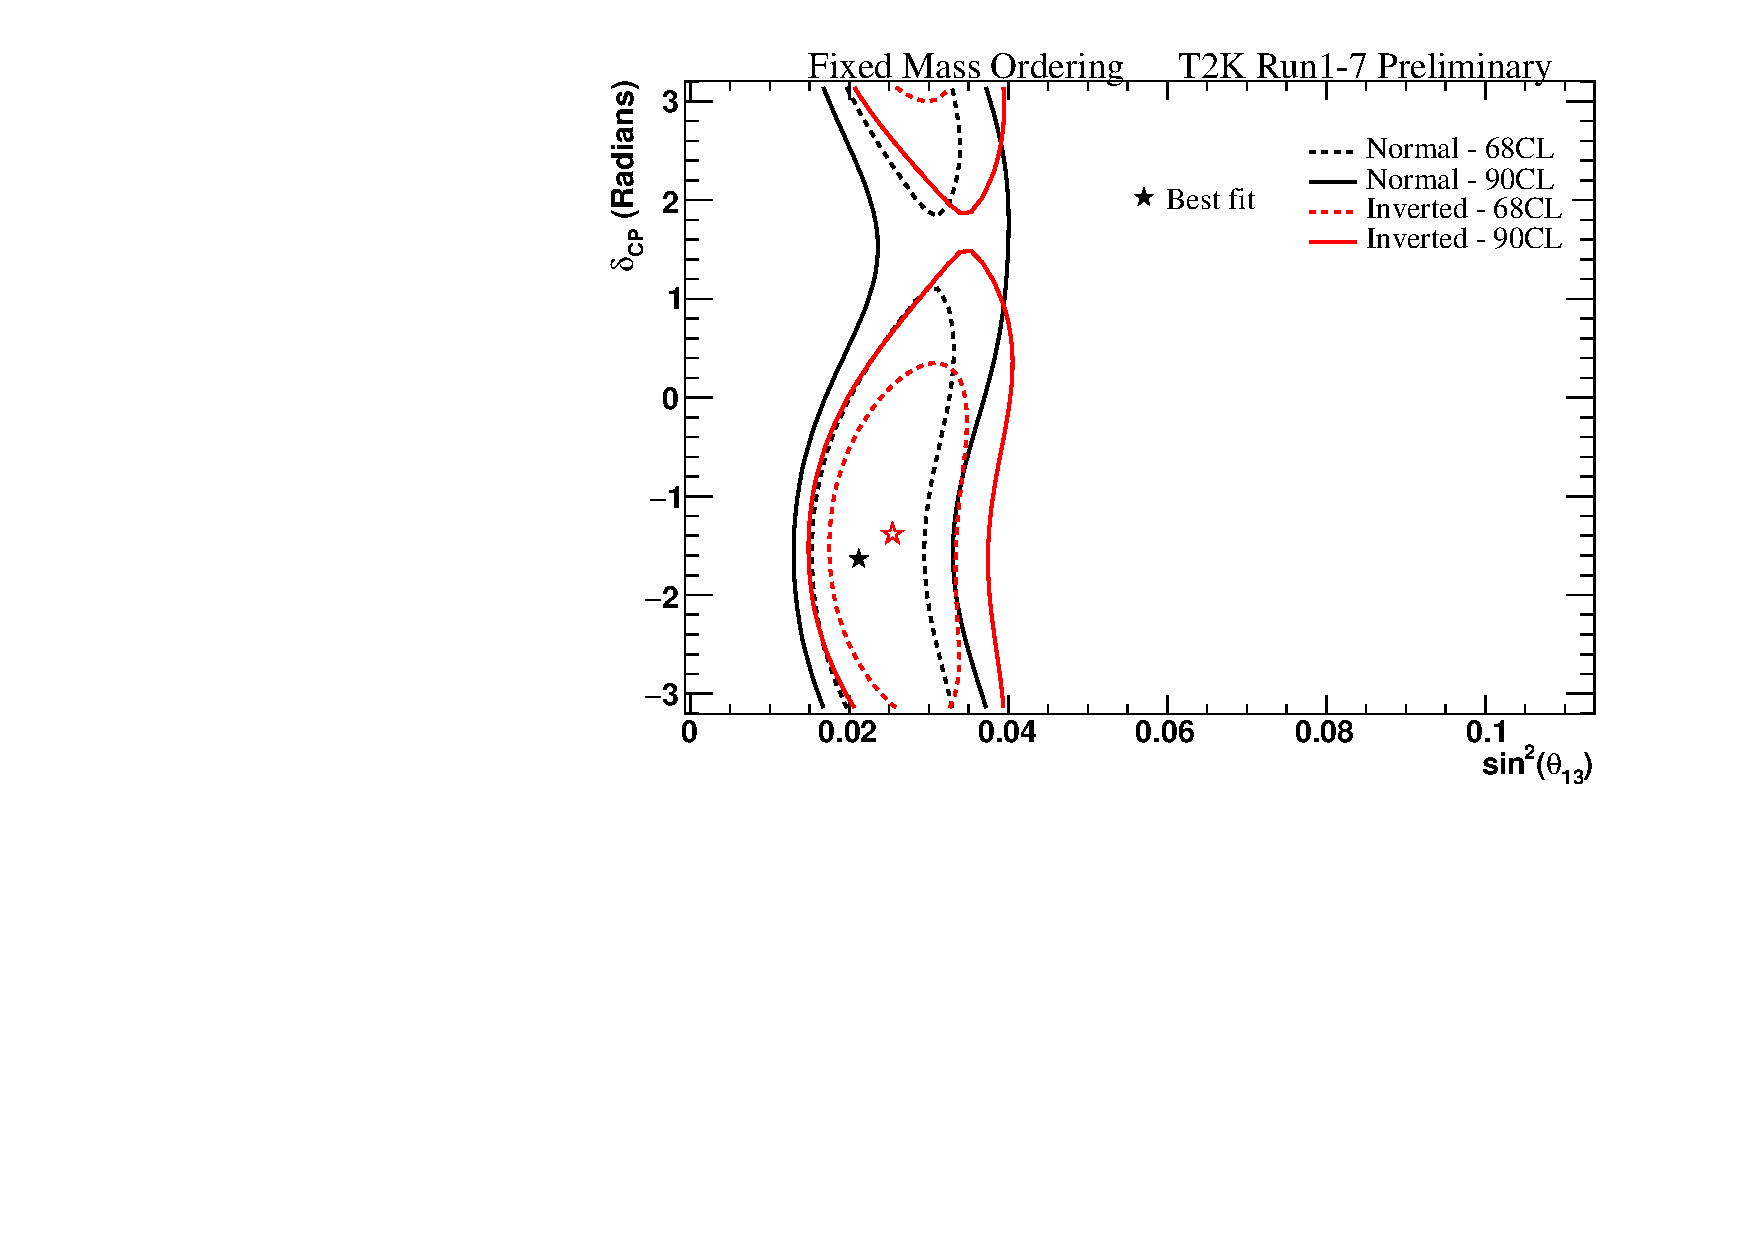
\includegraphics[trim={0cm 0cm 0cm 0cm}, clip, scale=0.33] {images/sensitivity/th13_dcp_global_t2k}
				\caption*{with reactor constraint}
			\end{figure}
		\end{column}
	\end{columns}
\end{frame}

\begin{frame}{\sinsqthetaonethree vs \deltacp sensitivity - Asimov B}
	\centering
	\begin{columns}
		\begin{column}{0.5\paperwidth}
			\begin{figure}
				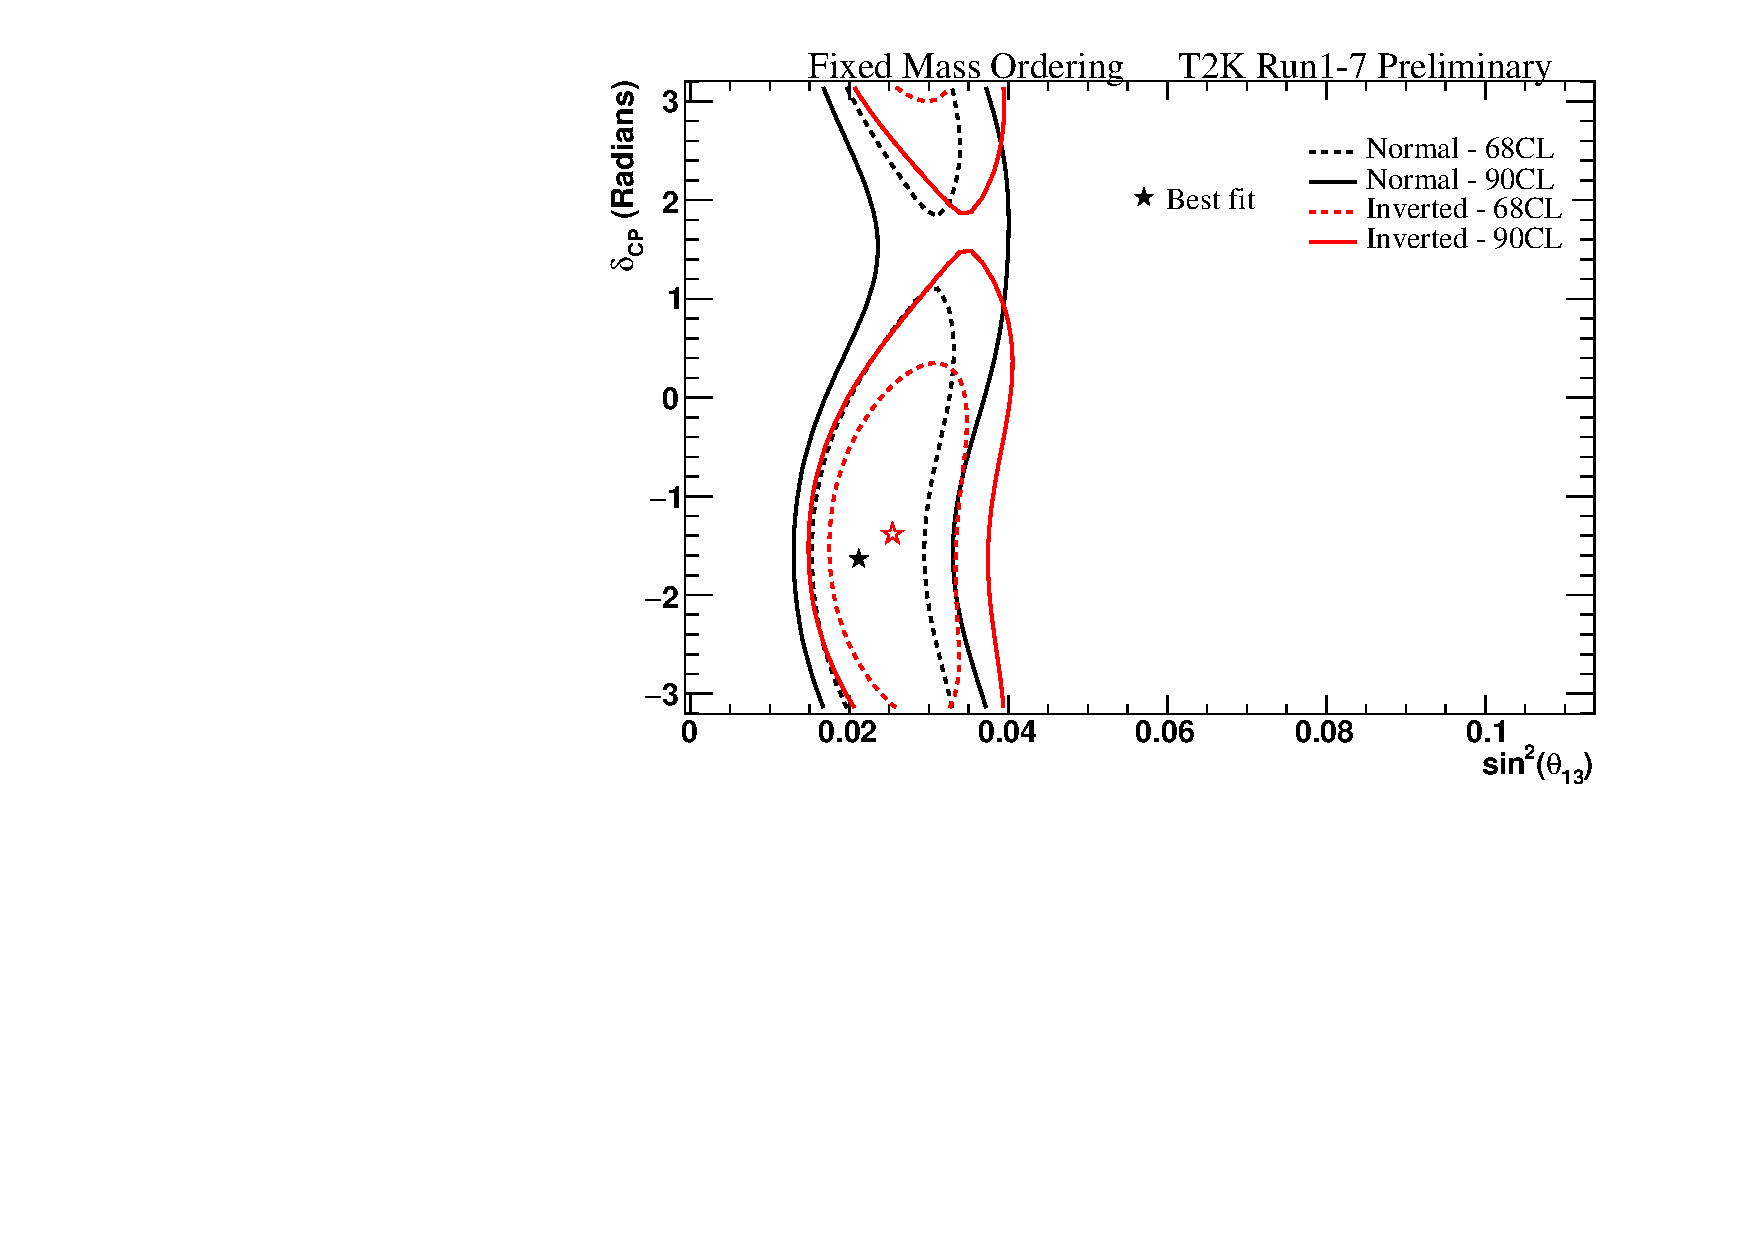
\includegraphics[trim={0cm 0cm 0cm 0cm}, clip, scale=0.33] {images/sensitivity/th13_dcp_global_t2k}
				\caption*{without reactor constraint}
			\end{figure}
		\end{column}
		\begin{column}{0.5\paperwidth}
			\begin{figure}
				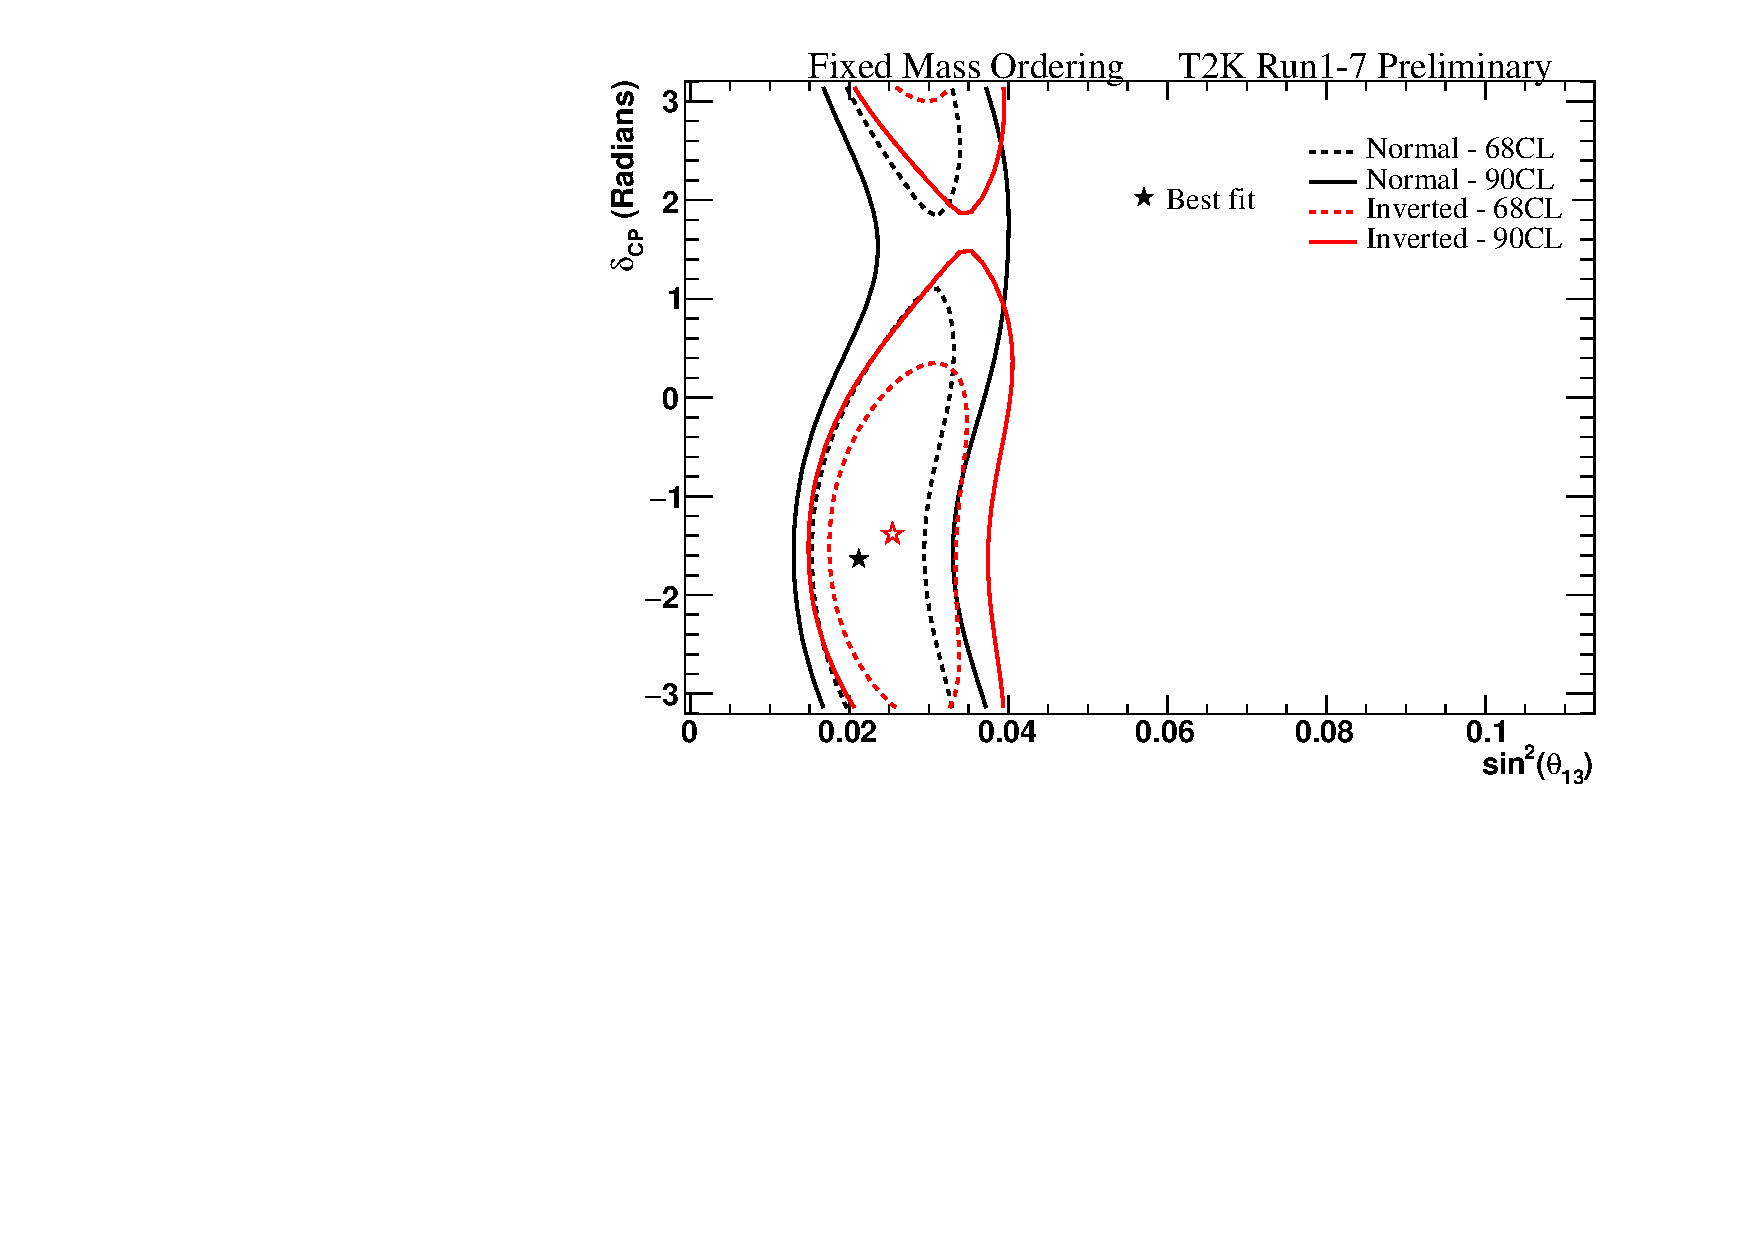
\includegraphics[trim={0cm 0cm 0cm 0cm}, clip, scale=0.33] {images/sensitivity/th13_dcp_global_t2k}
				\caption*{with reactor constraint}
			\end{figure}
		\end{column}
	\end{columns}
\end{frame}

%===============================================================================
\section{\sinsqthetatwothree vs \dmsqtwothree sensitivity}
\begin{frame}
	\centering
	\Large Run 1-8 \sinsqthetatwothree vs \dmsqtwothree sensitivity\\
\end{frame}

\begin{frame}{\sinsqthetatwothree vs \dmsqtwothree sensitivity - Asimov A}
	\centering
	\begin{columns}
		\begin{column}{0.5\paperwidth}
			\begin{figure}
				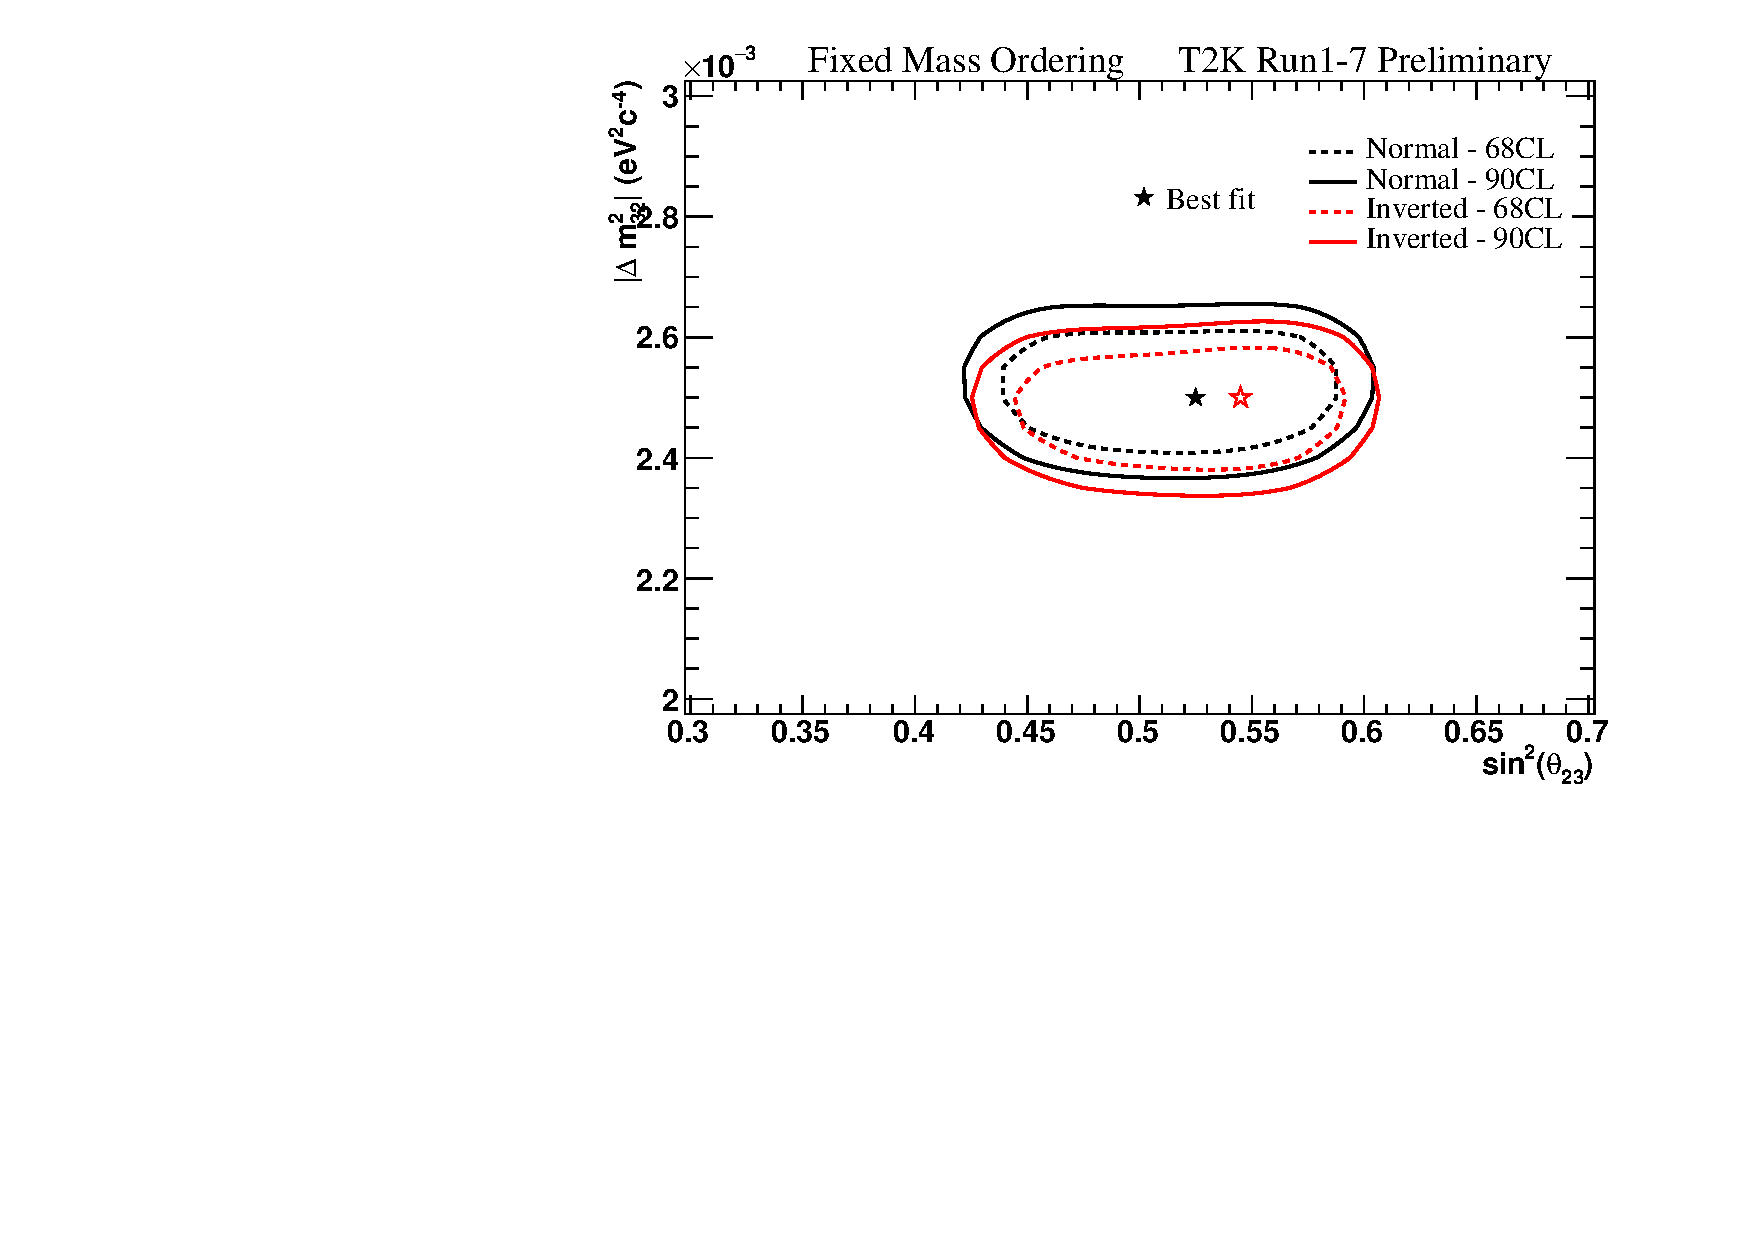
\includegraphics[trim={0cm 0cm 0cm 0cm}, clip, scale=0.33] {images/sensitivity/th23_dmsq23_global_t2k}
				\caption*{without reactor constraint}
			\end{figure}
		\end{column}
		\begin{column}{0.5\paperwidth}
			\begin{figure}
				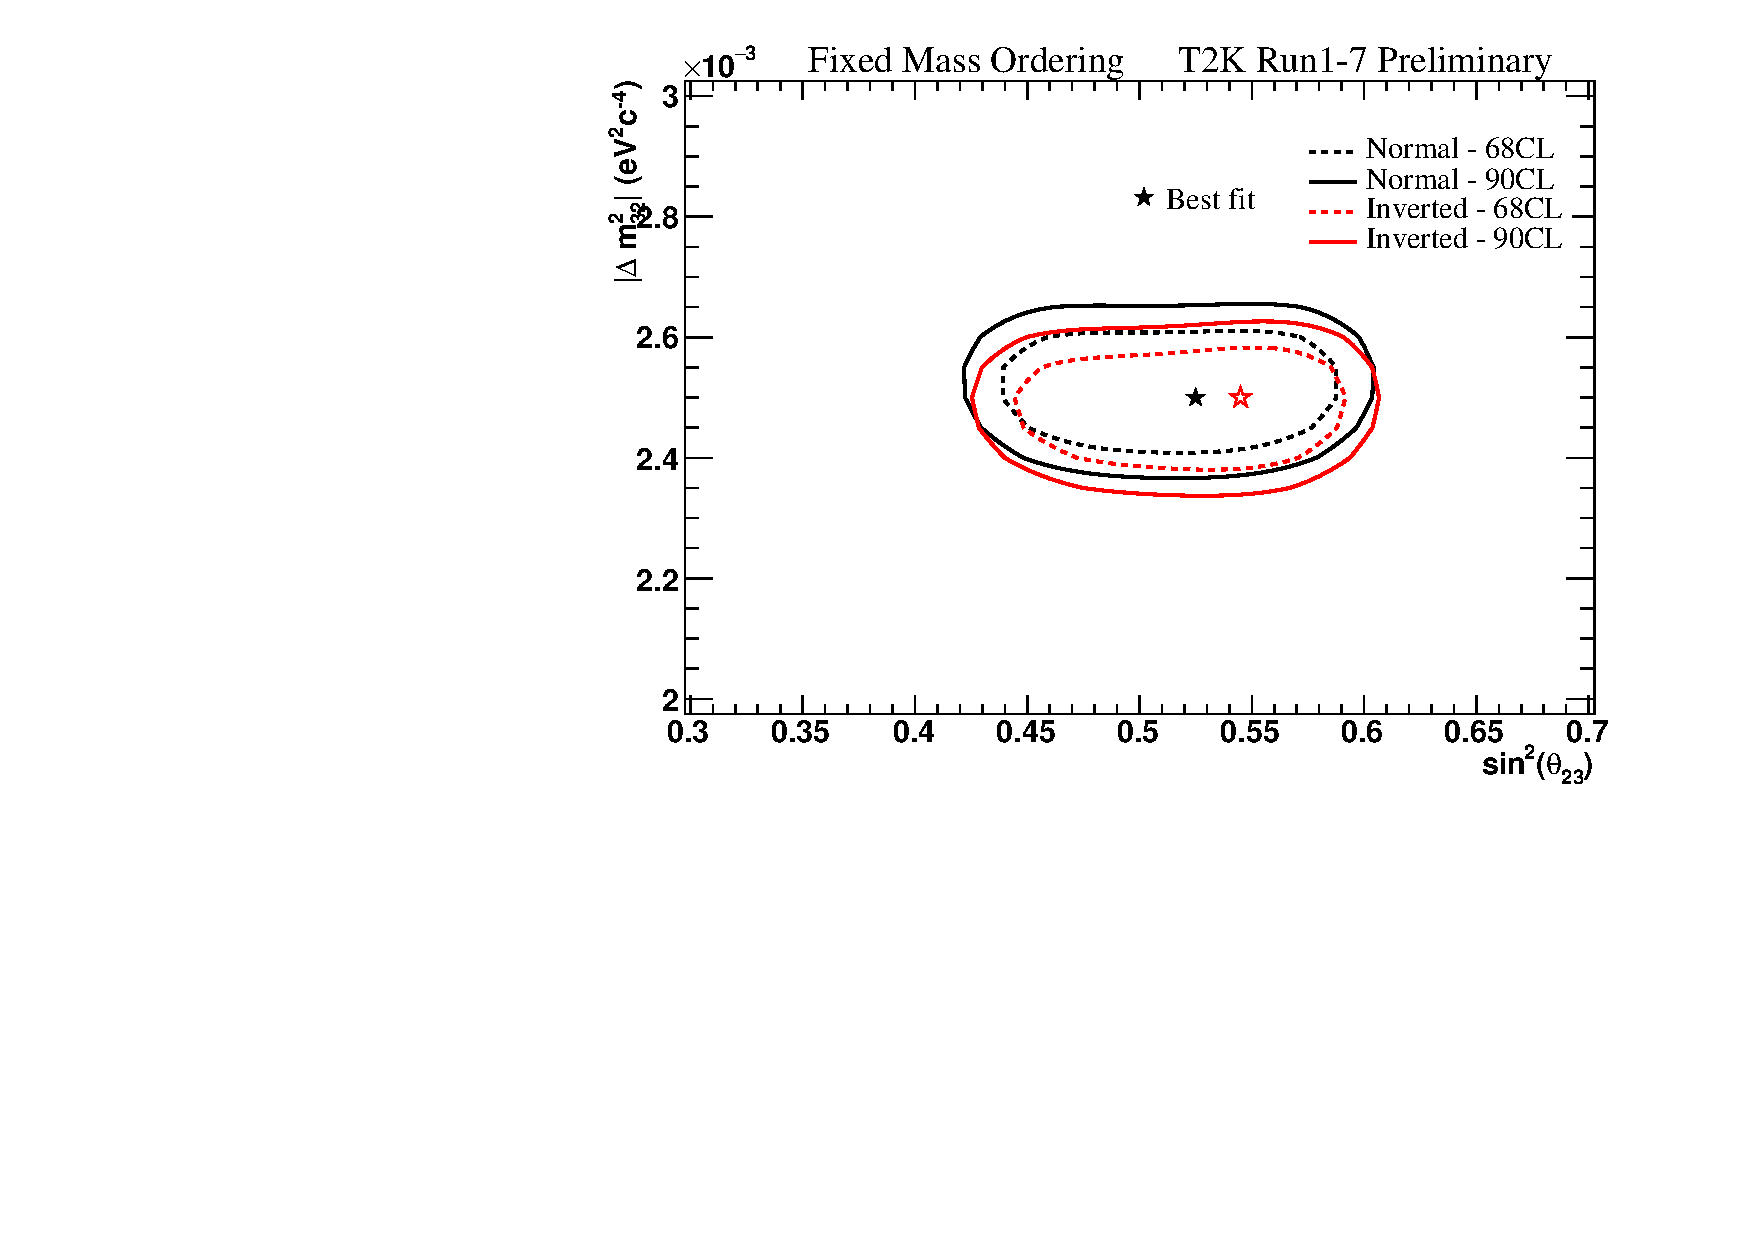
\includegraphics[trim={0cm 0cm 0cm 0cm}, clip, scale=0.33] {images/sensitivity/th23_dmsq23_global_t2k}
				\caption*{with reactor constraint}
			\end{figure}
		\end{column}
	\end{columns}
\end{frame}

\begin{frame}{\sinsqthetatwothree vs \dmsqtwothree sensitivity - Asimov B}
	\centering
	\begin{columns}
		\begin{column}{0.5\paperwidth}
			\begin{figure}
				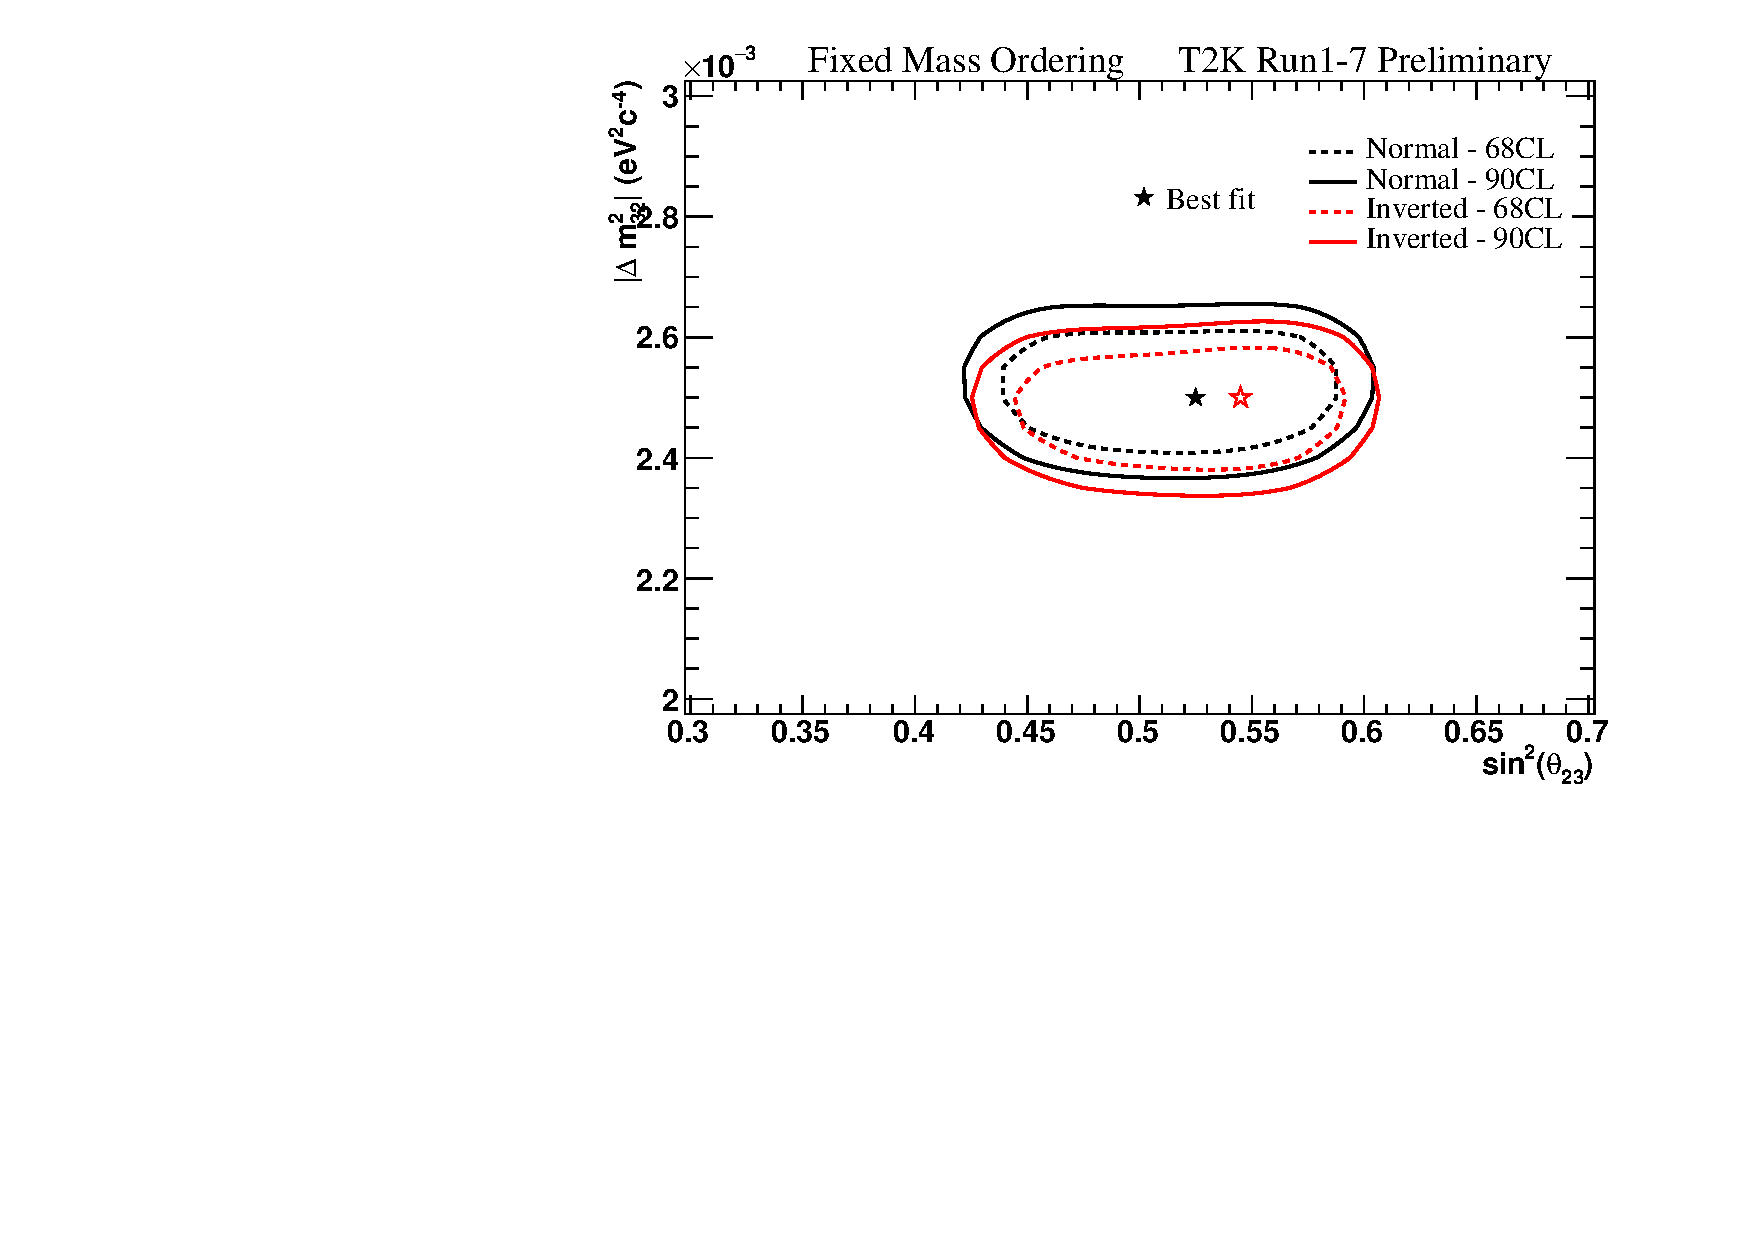
\includegraphics[trim={0cm 0cm 0cm 0cm}, clip, scale=0.33] {images/sensitivity/th23_dmsq23_global_t2k}
				\caption*{without reactor constraint}
			\end{figure}
		\end{column}
		\begin{column}{0.5\paperwidth}
			\begin{figure}
				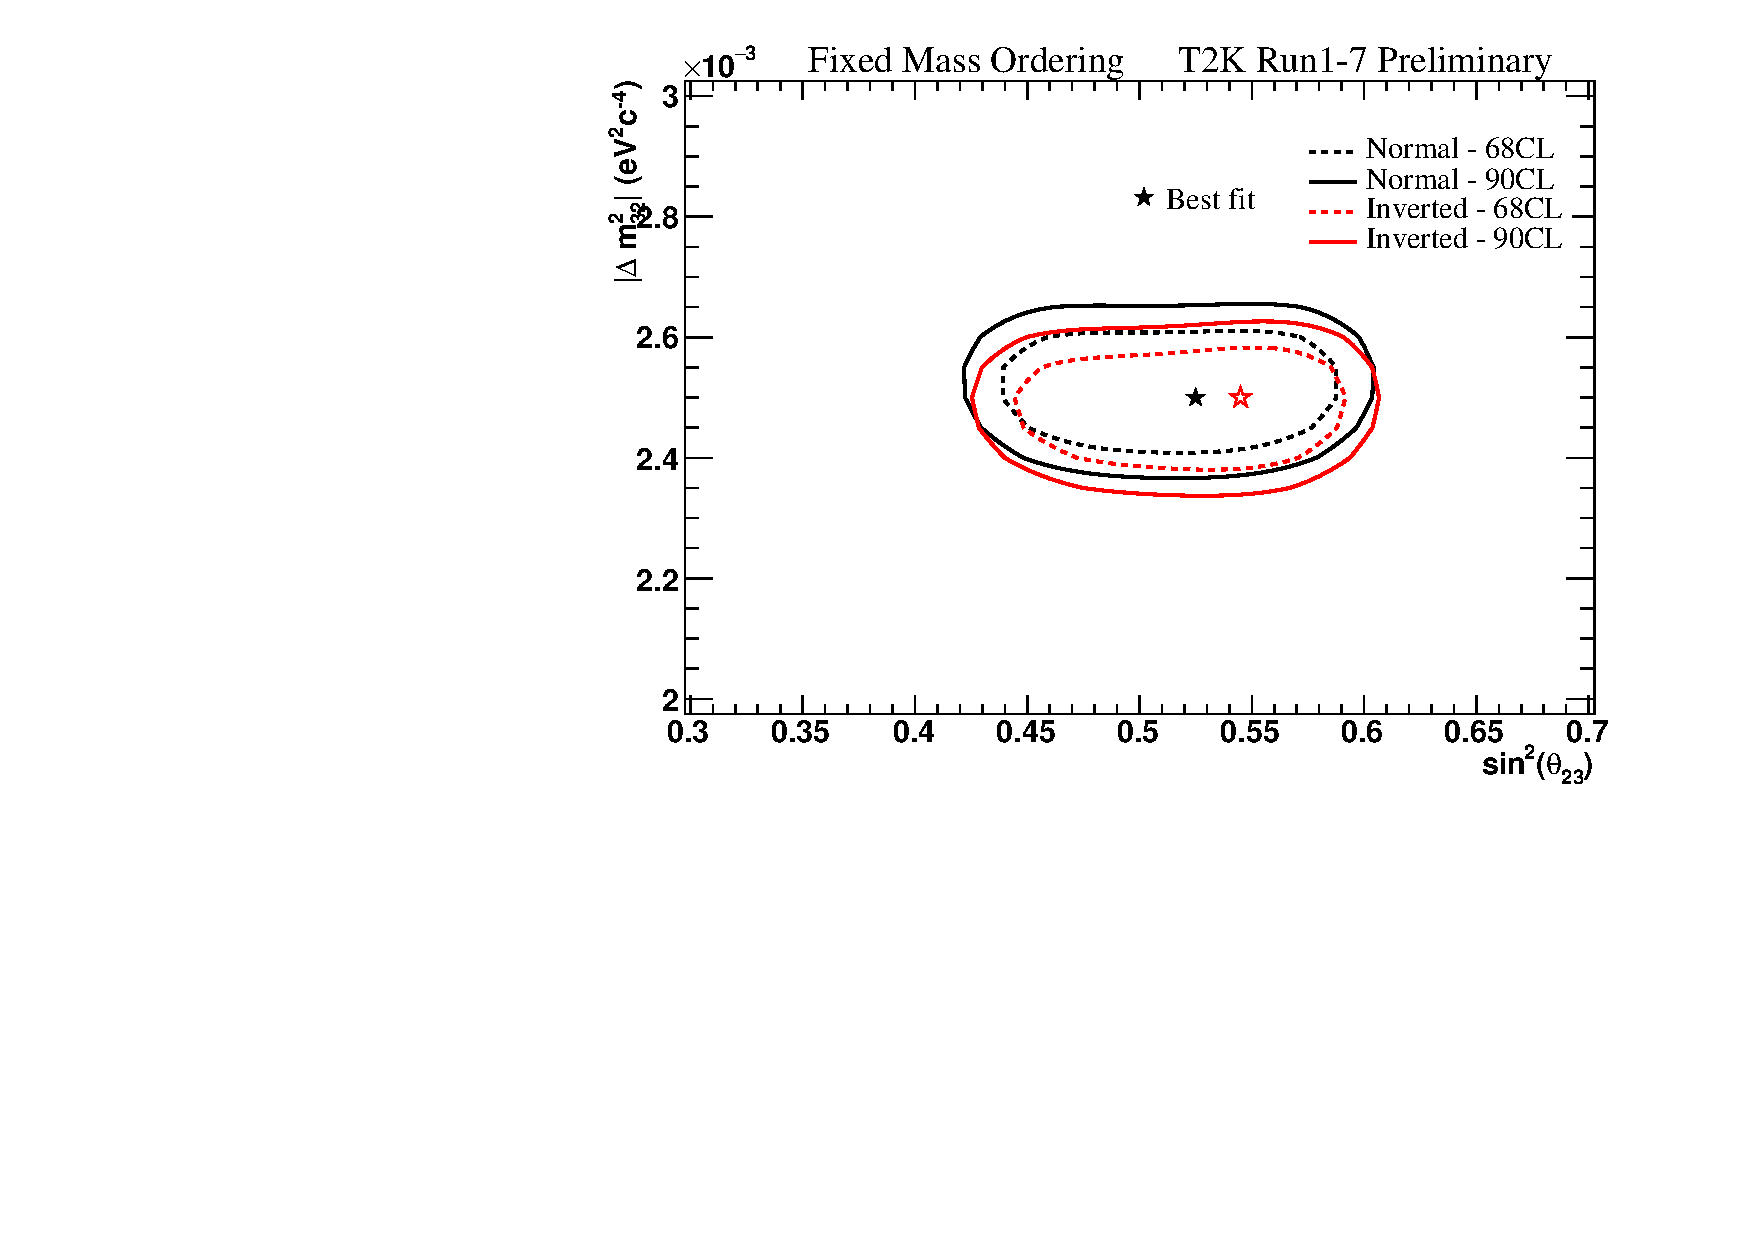
\includegraphics[trim={0cm 0cm 0cm 0cm}, clip, scale=0.33] {images/sensitivity/th23_dmsq23_global_t2k}
				\caption*{with reactor constraint}
			\end{figure}
		\end{column}
	\end{columns}
\end{frame}

%===============================================================================
\section{\sinsqthetatwothree vs \dmsqtwothree sensitivity}
\begin{frame}{Conclusion}
	\centering
	\begin{itemize}
		\item 
	\end{itemize}
\end{frame}

\end{document}

